\documentclass[conference]{IEEEtran}

\usepackage{pythonhighlight}
\documentclass{article}
\usepackage{graphicx}
\usepackage{subcaption} 
\usepackage{graphicx}
\usepackage{hyperref}
\usepackage{float}
\usepackage[english]{babel}
\usepackage{listings} % code blocks
\usepackage[utf8]{inputenc}
\usepackage{amsmath}
\usepackage[acronym]{glossaries}
\makeglossaries
%\usepackage{etoolbox} % citações

\hyphenation{}

\begin{document}
% paper title
% can use linebreaks \\ within to get better formatting as desired
\title{Twitter Sentiment Analysis}

% author names and affiliations
% use a multiple column layout for up to three different
% affiliations
\author{
    \IEEEauthorblockN{Nelson Loureiro}
   \IEEEauthorblockA{
        Fundamentos de Aprendizagem Automática 24/25\\
        Departamento de Eletrónica, Telecomunicações e Informática\\
        University of Aveiro\\
        Aveiro, Portugal\\
        nelson.loureiro@ua.pt
    }
    \and
    \IEEEauthorblockN{Cristiano Nicolau}
    \IEEEauthorblockA{
        Fundamentos de Aprendizagem Automática 24/25\\
        Departamento de Eletrónica, Telecomunicações e Informática\\
        University of Aveiro\\
        Aveiro, Portugal\\
        cristianonicolau@ua.pt
    }
}
% make the title area
\maketitle

\begin{abstract}
This project focuses on Twitter sentiment analysis using the "Twitter Entity Sentiment Analysis" dataset, which contains tweets categorized by their sentiment (e.g., positive, negative, neutral) towards specific entities. We implemented and evaluated a comprehensive suite of models to accurately classify tweet sentiment. These include traditional machine learning approaches such as Support Vector Machines (SVM) with Bag-of-Words (BoW) and TF-IDF features; lexicon-based methods like VADER and TextBlob; various Deep Learning (DL) architectures including Feed-Forward Neural Networks (FNNs), Convolutional Neural Networks (CNNs) for text, Long Short-Term Memory (LSTM) networks, Gated Recurrent Units (GRUs), and Bidirectional LSTMs (Bi-LSTMs); and the transformer-based model BERT. The models were developed with considerations for text pre-processing specific to Twitter data and hyperparameter tuning to optimize performance. This work has implications for applications in public opinion monitoring, brand reputation management, customer feedback analysis, and social media analytics.
\end{abstract}

\begin{center}
    \textit{\textbf{Keywords:} Twitter Sentiment Analysis, Natural Language Processing (NLP), Machine Learning, Deep Learning, Text Classification, SVM, LSTM, CNN, GRU, Bi-LSTM, BERT, VADER, TextBlob}
\end{center}
\IEEEpeerreviewmaketitle
%\acrlong{da}
%\acrshort{da}
%\acrfull{da}

\newacronym{ml}{ML}{Machine Learning}
\newacronym{svm}{SVM}{Support Vector Machine} 
\newacronym{mlp}{MLP}{Multi-layer Perceptrons}
\newacronym{fnn}{FNN}{Feedforward Neural Network}
\newacronym{TP}{TP}{True Positive}
\newacronym{FP}{FP}{False Positive}
\newacronym{TN}{TN}{True Negative}
\newacronym{FN}{FN}{False Negative}

\section{Introduction}
\label{sec:Introduction}
Sentiment analysis, the computational study of opinions, sentiments, and emotions expressed in text, is a vital domain in Natural Language Processing (NLP). It is used in a wide range of applications, such as brand monitoring, customer feedback analysis, political forecasting, and public opinion tracking. Analyzing sentiment on platforms like Twitter is particularly valuable due to the vast volume of real-time and user-generated content. Unlike generic text analysis, Twitter sentiment analysis involves navigating informal language, slang, abbreviations, emojis, and character limits, making it a challenging yet impactful task.

This paper aims at two key objectives. First, it provides a comprehensive review of the latest advances in Twitter sentiment analysis, critically analyzing and comparing other studies in the field. Second, it develops, optimizes, and evaluates a diverse set of modeling approaches using the "Twitter Entity Sentiment Analysis" dataset from Kaggle \cite{twitter_dataset}. This dataset comprises tweets annotated with sentiments towards various entities, posing a challenging multi-class sentiment classification problem.

Our study will explore different techniques in accurately classifying tweet sentiment. These include traditional machine learning approaches such as Support Vector Machines (SVM) with Bag-of-Words (BoW) and Term Frequency-Inverse Document Frequency (TF-IDF) features; lexicon-based methods like VADER and TextBlob; Deep Learning (DL) architectures including Feed-Forward Neural Networks (FNNs), Convolutional Neural Networks (CNNs) for text, Long Short-Term Memory (LSTM) networks, Gated Recurrent Units (GRUs), and Bidirectional LSTMs (Bi-LSTMs); and finally, transformer-based models like BERT. The paper concludes with a detailed comparative analysis of the model performances and offers key insights derived from the experiments.

\section{State of the Art} 
\label{sec}

A comprehensive state-of-the-art review was performed to identify the most suitable models for Twitter sentiment analysis and to survey existing studies applying similar techniques. The goal is to understand the strengths and weaknesses of various approaches when applied to the unique characteristics of Twitter data.

\subsection{Traditional Machine Learning Approaches}

Before the widespread adoption of deep learning, traditional machine learning algorithms were standard for sentiment analysis. These methods typically rely on handcrafted features extracted from the text.


\subsubsection{Support Vector Machines (SVM)}

Support Vector Machines (SVMs) have been widely used for text classification tasks, including sentiment analysis, due to their effectiveness in high-dimensional spaces and their ability to model non-linear decision boundaries. When applied to Twitter data, SVMs are often combined with feature representations like Bag-of-Words (BoW) or TF-IDF. For instance, Pang et al. (2002) \cite{pang2002thumbs}  demonstrated early success using SVMs for classifying movie reviews, laying foundational work for sentiment analysis. Later studies, such as Go et al. (2009) \cite{go2009twitter}, specifically adapted SVMs for Twitter sentiment classification by incorporating features like emoticons and N-grams, achieving good performance. The choice between BoW, which counts word occurrences, and TF-IDF, which weights words by their importance in the corpus, can significantly impact performance, with TF-IDF often providing more nuanced feature representations.


\subsection{Lexicon-Based Approaches}

Lexicon-based methods classify text sentiment based on the semantic orientation of words and phrases it contains, using pre-defined dictionaries or lexicons where words are scored for polarity (positive, negative, neutral) and sometimes intensity.


\subsubsection{VADER (Valence Aware Dictionary and sEntiment Reasoner)
}

VADER is a lexicon and rule-based sentiment analysis tool specifically attuned to sentiments expressed in social media. Hutto and Gilbert (2014) \cite{hutto2014vader} developed VADER to be particularly effective with microblogging content, as it considers lexical features common in such texts, like emoticons, slang, and degree modifiers (e.g., "very," "extremely"). It has been shown to perform well without requiring training data, making it a popular baseline.

\subsubsection{TextBlob}

TextBlob is a Python library for processing textual data, offering a straightforward API for common NLP tasks, including sentiment analysis. Its sentiment analysis module is based on a lexicon and a set of rules, providing polarity and subjectivity scores. While generally effective for well-structured text, its performance on noisy Twitter data can be less robust than specialized tools like VADER unless customized. Loria (2018) \cite{loria2018textblob} provides the foundation for TextBlob's functionalities.




\subsection{Feedforward Neural Networks (FNNs)}

Feedforward Neural Networks (FNNs), also known as Multi-Layer Perceptrons (MLPs), can be applied to sentiment analysis by taking word embeddings or other numerical text representations as input. While FNNs can learn complex patterns, they do not inherently capture the sequential nature of text as effectively as recurrent architectures. However, with appropriate feature engineering (e.g., using N-gram features or pre-trained word embeddings as input), FNNs can serve as effective classifiers. Zhang et al. (2015) \cite{zhang2015character} explored the use of character-level and word-level FNNs for text classification, highlighting their potential when combined with learned embeddings.

\subsection{Convolutional Neural Networks (CNNs)}


Convolutional Neural Networks (CNNs), initially designed for image processing, have been successfully adapted for text classification tasks. For text, 1D convolutions are applied over sequences of word embeddings to capture local patterns and N-gram features at different positions in the text. Kim (2014) \cite{kim2014convolutional} presented a work demonstrating the effectiveness of simple CNN architectures with pre-trained word embeddings for sentence-level classification tasks, including sentiment analysis. Subsequent research, such as Yin et al. (2017) \cite{yin2017comparative} in their comparative study, further explored various CNN architectures for text, showing their ability to learn hierarchical features from text data efficiently.



\subsection{Recurrent Neural Networks (RNNs)}

Recurrent Neural Networks are designed to process sequential data, making them naturally suited for text where word order and context are crucial.

\subsubsection{Long Short-Term Memory (LSTM)}

LSTMs, a type of RNN introduced by Hochreiter and Schmidhuber (1997) \cite{hochreiter1997long}, are specifically designed to overcome the vanishing gradient problem, allowing them to learn long-range dependencies in text. LSTMs have become a popular choice for sentiment analysis. Wang et al. (2016) \cite{wang2016ataelstm} demonstrated the utility of LSTMs for Twitter sentiment analysis, often using pre-trained word embeddings like Word2Vec or GloVe as input to the embedding layer.

\subsubsection{Gated Recurrent Units (GRU)}

GRUs, introduced by Cho et al. (2014) \cite{cho2014learning}, are a variation of LSTMs that simplify the gate mechanism, having fewer parameters and thus sometimes training faster while achieving comparable performance. GRUs are also effective for capturing sequential information in text and have been applied to Twitter sentiment analysis, often showing similar results to LSTMs as noted by Chung et al. (2014) \cite{chung2014empirical} in their empirical evaluation.


\subsubsection{Bidirectional LSTMs (Bi-LSTM)
}

Bidirectional LSTMs process text in both forward and backward directions, allowing the model to capture context from past and future words simultaneously. This can lead to a richer understanding of the text and improved performance in sentiment analysis tasks. Schuster and Paliwal (1997) \cite{schuster1997bidirectional} introduced the concept of bidirectional RNNs. Many studies, such as Brahmbhatt et al. (2019) \cite{brahmbhatt2019comparative}, have shown that Bi-LSTMs often outperform unidirectional LSTMs on various NLP tasks, including Twitter sentiment analysis, by providing a more complete contextual representation.

\subsection{Transformer-Based Models (BERT)
}


Transformer models, particularly BERT (Bidirectional Encoder Representations from Transformers) developed by Devlin et al. (2019) \cite{devlin2019bert}, have revolutionized the NLP landscape. BERT is pre-trained on vast amounts of text data and can be fine-tuned for specific tasks, including sentiment analysis, achieving state-of-the-art results. BERT's attention mechanism allows it to weigh the importance of different words when representing a sentence, capturing complex contextual relationships.Several studies have demonstrated BERT's effectiveness for Twitter sentiment analysis, often outperforming previous LSTM and CNN-based approaches, although they are computationally more intensive. This can be observed in \cite{article}, which presents a comparative analysis of various studies evaluating different models on Twitter sentiment tasks.  Variants like RoBERTa and specialized Twitter-BERT models (e.g., BERTweet by Nguyen et al. (2020) \cite{nguyen2020bertweet}) have further pushed performance boundaries on social media text.


\section{Machine Learning and Deep Learning Models for Sentiment Analysis}
\label{sec:ML_DL_Models}

\subsection{Introduction}
In this section, we present and discuss the machine learning and deep learning models implemented in this project, focusing on their structure, functionality, and contributions to the problem of Twitter sentiment analysis. These models fall within the supervised learning paradigm, with some lexicon-based approaches also explored, and are specifically chosen to address the challenges inherent in classifying sentiment from short, informal, and often noisy text data from Twitter.

We begin with an exploration of traditional Machine Learning (ML) models like Support Vector Machines (SVMs) using Bag-of-Words (BoW) and TF-IDF features. We then discuss lexicon-based approaches such as VADER and TextBlob. Following this, we delve into several neural network architectures, including Feedforward Neural Networks (FNNs), Convolutional Neural Networks (CNNs) adapted for text, and various Recurrent Neural Networks (RNNs) like Long Short-Term Memory (LSTM), Gated Recurrent Units (GRU), and Bidirectional LSTMs (Bi-LSTMs). Finally, we cover the powerful transformer-based model, BERT.

Each model leverages unique mechanisms to process and learn from textual data, enabling accurate classification of tweet sentiment. Furthermore, we describe the text pre-processing steps, feature extraction techniques, and hyperparameter tuning strategies employed to optimize these models for enhanced performance. The discussion also touches upon how data characteristics unique to Twitter are handled.

Finally, we outline the evaluation metrics and hyperparameters used to assess the models’ effectiveness. These metrics provide a comprehensive understanding of the models’ predictive accuracy, robustness, and suitability for the sentiment classification task at hand.

\subsection{Traditional Machine Learning Approaches}

\subsubsection{Support Vector Machines (SVM)}
Support Vector Machines are supervised learning models renowned for their effectiveness in classification tasks, particularly in high-dimensional spaces. The core idea of SVM is to find an optimal hyperplane that best separates data points belonging to different classes in the feature space. For non-linearly separable data, SVMs can use a "kernel trick" (e.g., polynomial, radial basis function (RBF) kernels) to map data into a higher-dimensional space where a linear separation becomes possible.

\begin{figure} [h!]
    \centering
    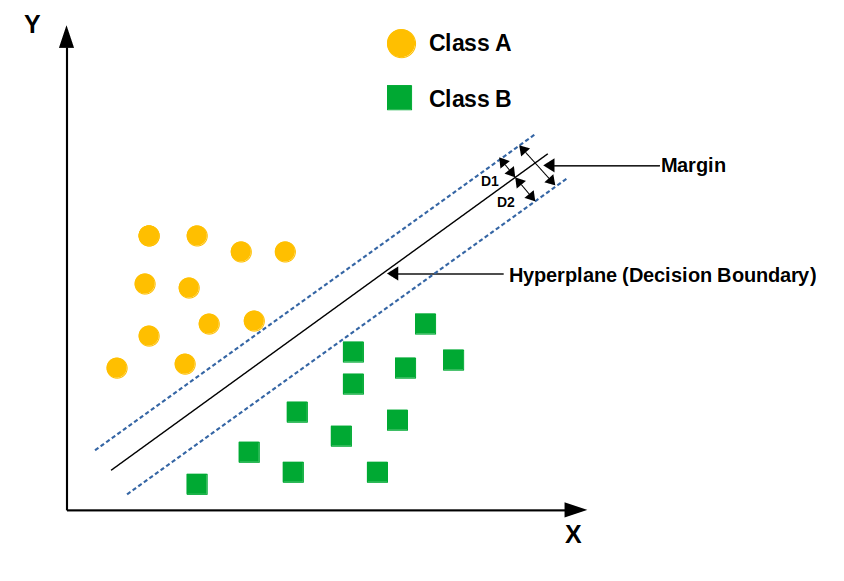
\includegraphics[width=0.75\linewidth]{images/svm_arch.png}
    \caption{SVM Structure}
    \label{fig:enter-label}
\end{figure}

For Twitter sentiment analysis, SVMs are typically used with text features extracted using methods like:

\begin{itemize}
    \item Bag-of-Words (BoW): This approach represents text by the occurrence of words within it, disregarding grammar and word order but keeping multiplicity. Each tweet is converted into a vector where each dimension corresponds to a word in the vocabulary, and the value can be the count of the word or a binary indicator of its presence.
    \item Term Frequency-Inverse Document Frequency (TF-IDF): TF-IDF is a numerical statistic that reflects how important a word is to a document (a tweet, in this case) in a collection or corpus. It increases proportionally to the number of times a word appears in the document but is offset by the frequency of the word in the corpus. This helps to give more weight to words that are frequent in a tweet but not frequent across all tweets.
\end{itemize}

SVMs trained on BoW or TF-IDF features have demonstrated strong performance in many text classification tasks, including sentiment analysis, by effectively navigating the sparsity and high dimensionality of such data.

\subsection{Lexicon-Based Approaches}
Lexicon-based approaches classify sentiment based on the semantic orientation of words and phrases present in the text. They rely on a sentiment lexicon, which is a dictionary of words pre-annotated with their sentiment scores (e.g., positive, negative, neutral) and sometimes intensity.

\subsubsection{VADER (Valence Aware Dictionary and Sentiment Reasoner)}
VADER is a lexicon and rule-based sentiment analysis tool specifically attuned to sentiments expressed in social media. It considers lexical features common in microblogging, such as emoticons, slang, acronyms, and degree modifiers (e.g., "very," "extremely"). VADER produces a sentiment score (compound score) that indicates both the polarity (positive/negative) and intensity of the sentiment. It is particularly useful for analyzing Twitter data due to its focus on social media language and its ability to perform well without training data.

\subsubsection{TextBlob}
TextBlob is a Python library providing a simple API for common NLP tasks, including sentiment analysis. Its sentiment analysis functionality is built upon a lexicon (often based on WordNet) and a set of rules to determine sentiment polarity (ranging from -1 to 1) and subjectivity (ranging from 0 to 1). While easy to use, its general-purpose lexicon might be less effective on nuanced or domain-specific Twitter language compared to VADER unless customized.

\subsection{Feedforward Neural Networks (FNN)}
A Feedforward Neural Network (FNN) is one of the simplest forms of artificial neural networks. It is designed to approximate functions by mapping input data to output labels through a series of hidden layers. FNNs process information in one direction—from the input layer, through the hidden layers, to the output layer—without forming cycles or loops.

\begin{figure}[h!]
    \centering
    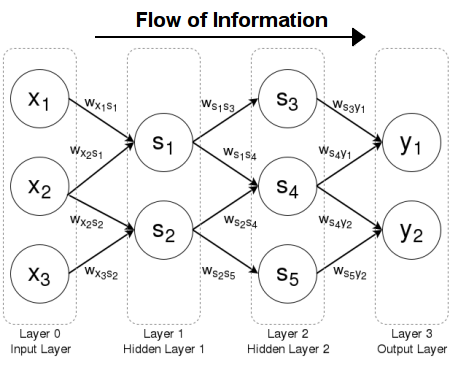
\includegraphics[width=0.8\linewidth]{images/fnn-str.png}
    \caption{Structure of a Feedforward Neural Network}
    \label{fig:feedforward_structure}
\end{figure}

Each neuron in an FNN applies a weighted sum to its inputs, adds a bias, and passes the result through an activation function:
$$
y = f\left(\sum_{i=1}^{n} w_i x_i + b\right)
$$
where (y) is the output, (x\_i) are inputs, (w\_i) are weights, (b) is bias, and (f) is an activation function (e.g., ReLU, Sigmoid).

An FNN consists of:

\begin{itemize}
    \item Input Layer: Receives input features. For text, these features are often word embeddings (dense vector representations of words) or TF-IDF vectors.
    \item Hidden Layers: Perform transformations using weights, biases, and activation functions. The depth and width of these layers determine the model's capacity.
    \item Output Layer: Produces predictions. For sentiment classification (e.g., positive, negative, neutral), a Softmax activation function is typically used to output class probabilities.
\end{itemize}


\begin{figure}[H]
    \centering
    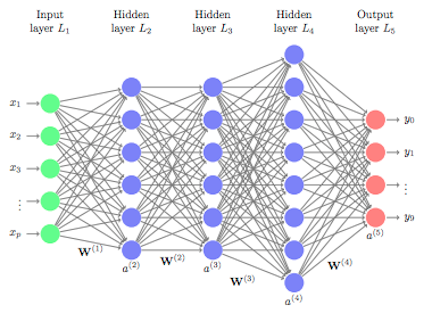
\includegraphics[width=1\linewidth]{images/feedforward_workflow.png}
    \caption{Workflow of a Feedforward Neural Network}
    \label{fig:feedforward_workflow}
\end{figure}

The workflow involves forward propagation (calculating output), loss calculation (measuring error), backpropagation (calculating gradients), and optimization (updating weights).

For text classification, FNNs can be effective when used with appropriate input representations like pre-trained word embeddings (e.g., Word2Vec, GloVe, FastText) or TF-IDF vectors. While they don't inherently capture sequential information like RNNs or local contextual patterns like CNNs for text, they can serve as strong classifiers on aggregated or transformed text features.

\subsection{Convolutional Neural Networks (CNN) for Text}
While traditional Neural Networks like FNNs can struggle with the high dimensionality and local structure of raw text, Convolutional Neural Networks (CNNs), originally designed for image processing, have been successfully adapted for text classification tasks. Instead of applying 2D convolutions to image pixels, 1D convolutions are applied over sequences of word embeddings.

\begin{figure}[h!]
    \centering
    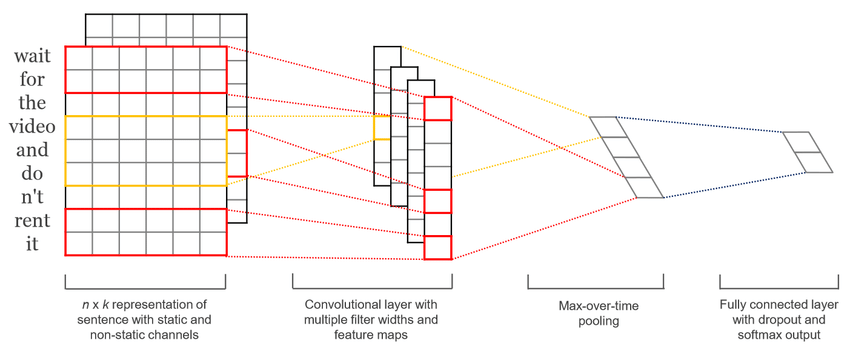
\includegraphics[width=0.75\linewidth]{images/cnn-struture.png}
    \caption{CNN Struture (Text Example}
    \label{fig:enter-label}
\end{figure}

In this context:

\begin{itemize}
    \item Input Representation: Tweets are first converted into a matrix where each row represents a word and columns represent the dimensions of its word embedding (e.g., from Word2Vec, GloVe, or learned during training).
    \item Convolutional Layer: 1D filters (kernels) of different lengths (e.g., spanning 2, 3, or 4 words at a time, akin to n-grams) slide across the sequence of word embeddings. Each convolution operation produces a feature. The idea is that these filters learn to detect meaningful patterns or n-grams relevant to sentiment (e.g., "very good," "not bad").
    \item Activation Function: A non-linear activation function like ReLU is applied to the output of the convolutions.
    \item Pooling Layer: A 1D max-over-time pooling operation is typically applied to the feature maps generated by the convolutional layer. This takes the maximum value over the time (sequence) dimension for each filter, effectively capturing the most salient feature detected by that filter across the entire tweet. This also results in a fixed-size output vector, regardless of the input tweet length.
    \item Fully Connected Layer: The pooled features from various filters are concatenated and fed into one or more fully connected layers, culminating in an output layer (e.g., with Softmax activation) for sentiment classification.
\end{itemize}
CNNs for text are effective at capturing local contextual information and hierarchical features from text data. They are computationally less expensive than some RNN variants and can be very powerful, especially when combined with pre-trained word embeddings.


\subsection{Recurrent Neural Networks (RNN)}
Recurrent Neural Networks are specifically designed for processing sequential data like text, where the order of elements (words) is crucial. Unlike FNNs, RNNs have connections that form directed cycles, allowing them to maintain an internal state or "memory" of past information while processing a sequence.

\subsubsection{Long Short-Term Memory (LSTM)}
Standard RNNs suffer from the vanishing gradient problem, making it difficult for them to learn long-range dependencies in sequences. LSTMs address this issue through a more complex recurrent unit containing three "gates":

\begin{itemize}
    \item Input Gate: Controls how much of the new input is let into the memory cell.
    \item Forget Gate: Controls how much of the existing memory cell content is forgotten.
    \item Output Gate: Controls how much of the memory cell content is passed to the output and the next hidden state.
\end{itemize}

These gates allow LSTMs to selectively remember or forget information over long sequences, making them highly effective for tasks like sentiment analysis where context from earlier parts of a sentence (or tweet) can influence the overall sentiment.

\subsubsection{Gated Recurrent Units (GRU)}
GRUs are a variation of LSTMs that simplify the gating mechanism. They have two gates:

\begin{itemize}
    \item Reset Gate: Determines how to combine the new input with the previous memory.
    \item Update Gate: Determines how much of the previous memory to keep.
\end{itemize}

GRUs often achieve performance comparable to LSTMs on many tasks but with fewer parameters, potentially leading to faster training and less overfitting on smaller datasets.

\subsubsection{Bidirectional LSTMs (Bi-LSTM)}
Standard LSTMs (and GRUs) process sequences in one direction (e.g., from left to right). However, the sentiment of a tweet can depend on context from both preceding and succeeding words. Bidirectional LSTMs address this by using two separate LSTM layers: one processes the input sequence from start to end (forward layer), and the other processes it from end to start (backward layer). The outputs from both layers at each time step are typically concatenated (or combined in other ways) before being passed to the next layer. This allows the model to have a more complete understanding of the context of each word in the tweet. Bi-LSTMs often outperform unidirectional LSTMs in sentiment analysis tasks.

\subsection{BERT (Bidirectional Encoder Representations from Transformers)}
BERT represents a significant advancement in NLP, leveraging the Transformer architecture, which relies heavily on a mechanism called self-attention. Unlike RNNs that process words sequentially, Transformers process all words in a sequence simultaneously, allowing the model to weigh the importance of different words when representing each word in its context.

Key aspects of BERT include:

\begin{itemize}
    \item Pre-training: BERT is pre-trained on massive amounts of unlabeled text data (like Wikipedia and BooksCorpus) using two unsupervised tasks: Masked Language Model (MLM) and Next Sentence Prediction (NSP). This allows BERT to learn rich, deep bidirectional representations of language.
    \item Bidirectionality: Unlike earlier models like GPT (which were unidirectional), BERT's self-attention mechanism allows it to consider both left and right context for every word in a sequence from the very beginning of pre-training.
    \item Fine-tuning: After pre-training, BERT can be fine-tuned for various downstream NLP tasks, including sentiment analysis, by adding a small task-specific output layer and training on labeled data. For sentiment classification, a classification layer is typically added on top of the [CLS] token's output representation from BERT.
    \item 
\end{itemize}
BERT and its variants (e.g., RoBERTa, ALBERT, DistilBERT, and domain-specific versions like BERTweet for Twitter data) have achieved state-of-the-art results on many NLP benchmarks. For Twitter sentiment analysis, fine-tuning a pre-trained BERT model can yield very strong performance by leveraging its robust understanding of language nuances.

\subsection{Text Pre-processing, Data Augmentation for Text and Hyperparameter Tuning}

To enhance the performance and generalization of the sentiment analysis models, this study employs several techniques.

\subsubsection{Text Pre-processing}
Twitter data is notoriously noisy, containing slang, misspellings, abbreviations, URLs, mentions (@username), hashtags (\#topic), and emoticons. Effective pre-processing is crucial:

\begin{itemize}
    \item \textbf{Cleaning}: Removing URLs, mentions, special characters (while retaining sentiment-bearing ones like emoticons or punctuation like '!'), and HTML tags.
    \item \textbf{Normalization}: Converting text to lowercase, correcting common misspellings or slang (e.g., "u" to "you"), expanding contractions (e.g., "can't" to "cannot").
    \item \textbf{Tokenization}: Splitting tweets into individual words or sub-word units.
    \item \textbf{Stop Word Removal}: Optionally removing common words (e.g., "the," "is," "in") that may not carry significant sentiment, although this can sometimes be detrimental if not done carefully (e.g., "not" is a stop word but crucial for sentiment).
    \item \textbf{Lemmatization/Stemming}: Reducing words to their root form (e.g., "running" to "run"). Lemmatization is generally preferred as it results in actual words.
\end{itemize}

\subsubsection{Data Augmentation for Text}
Data augmentation for text aims to artificially increase the diversity of the training dataset. While not as straightforward as image augmentation, common techniques include:

\begin{itemize}
    \item \textbf{Synonym Replacement}: Randomly replacing words with their synonyms (e.g., using WordNet).
    \item \textbf{Random Insertion}: Inserting random synonyms of words at random positions.
    \item \textbf{Random Deletion}: Randomly deleting words from a sentence.
    \item \textbf{Back-Translation}: Translating a sentence to another language and then back to the original, which can create paraphrased versions.
\end{itemize}

\subsubsection{Hyperparameter Tuning}
Hyperparameter tuning involves systematically optimizing the parameters that govern the training process and architecture of the models. 

By integrating thorough text pre-processing and hyperparameter tuning into the modeling workflow, the implemented models are better equipped to handle the challenges of Twitter sentiment analysis, yielding improved accuracy and robustness in their predictions.

\subsection{Model Evaluation: Confusion Matrix and Classification Metrics}

The evaluation of the sentiment analysis models will be carried out using the confusion matrix, which provides a detailed view of the model’s correct and incorrect predictions for each sentiment class (e.g., positive, negative, neutral). In addition, classification metrics including \textit{accuracy}, \textit{precision}, \textit{recall}, and \textit{F1-score} will be calculated. These metrics are essential for assessing the effectiveness of the model in differentiating between various sentiment types.

\subsubsection{Confusion Matrix}

A confusion matrix is a table that indicates the mistakes and successes of your model, comparing to the expected result. The layout of a confusion matrix is present on the next figure. We will utilize the confusion\_matrix function from scikit-learn.

\begin{figure}[h!]
    \centering
    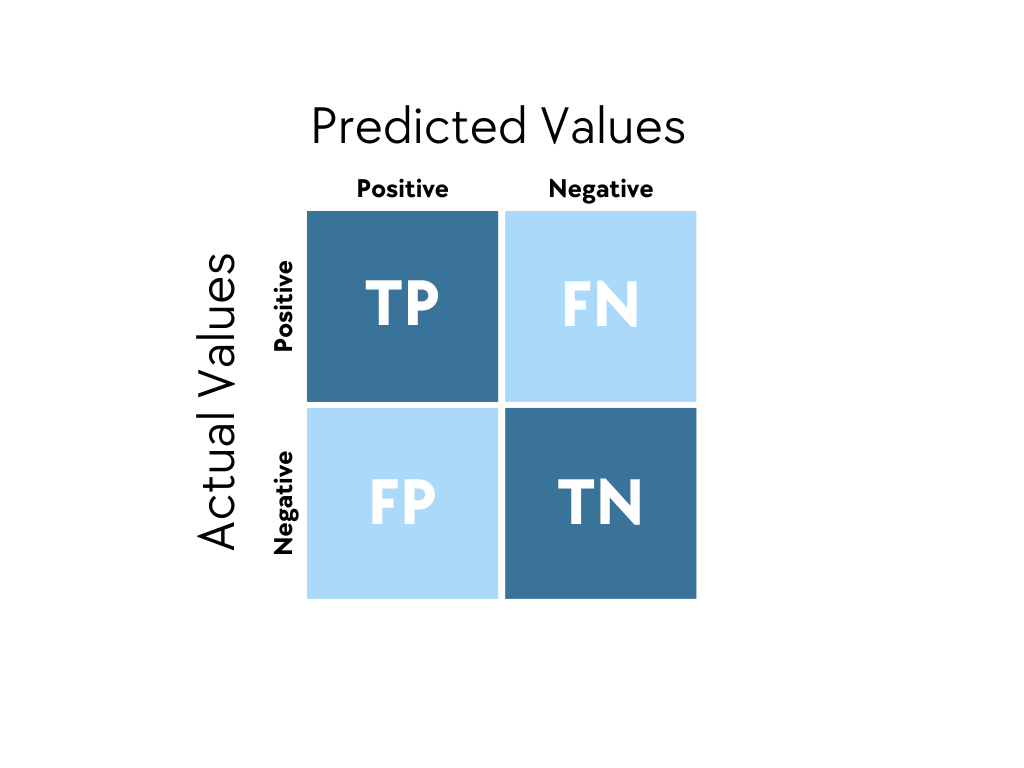
\includegraphics[width=1\linewidth]{images/confusion-matrix.png}
    \caption{Confusion Matrix}
    \label{fig:confusion_matrix}
\end{figure}

\subsubsection{Precision}
Precision measures the ratio of true positive predictions to the total number of positive predictions made by the model. It answers the question: "Of all tweets predicted as positive, how many were actually positive?"
$$Precision=\frac{True Positives (TP)}{True Positives (TP)+False Positives (FP)}$$

\subsubsection{Recall (Sensitivity)}
Recall (or sensitivity, or True Positive Rate) gauges the model’s ability to correctly identify all relevant instances from the total number of actual positive instances in the dataset. It answers: "Of all actual positive tweets, how many did the model correctly predict as positive?"
$$Recall=\frac{True Positives (TP)}{True Positives (TP)+False Negatives (FN)}$$

\subsubsection{F1-Score}
The F1-score is the harmonic mean of precision and recall, providing a balanced assessment of a model’s performance, especially useful when class distributions are imbalanced.
$$F1Score=2 \times \frac{Precision \times Recall}{Precision+Recall}$$

\subsubsection{Accuracy}
Accuracy is the proportion of correct predictions (both true positives and true negatives for binary, or sum of correct predictions across all classes for multi-class) to the total number of predictions made. It represents the overall correctness of the model's predictions.
$$Accuracy= \frac{\text{Number of Correct Predictions}}{\text{Total Number of Predictions}}$$


\subsubsection{Training Loss}
Training loss quantifies how well the model fits the training data by calculating the difference between predicted and actual values using a loss function (e.g., cross-entropy for classification). A lower loss generally indicates better model fit. The goal during training is to minimize this loss, though monitoring validation loss is crucial to prevent overfitting.

\section{Preprocessing and Data Visualization}
\label{sec:DatasetAndPreprocessing}

\subsection{Dataset Description}

This project utilizes the "Twitter Entity Sentiment Analysis" dataset from Kaggle \cite{twitter_dataset}. This dataset provides a collection of tweets, each associated with a specific entity and annotated with a sentiment label, serving as a robust foundation for training and evaluating sentiment analysis models.

The raw data for training and validation was initially loaded with columns subsequently renamed for clarity to: `tweetID`, `entity`, `sentiment`, and `tweet\_content`.

The initial preparation steps involved:
\begin{enumerate}
    \item \textbf{Standardizing Sentiment Labels}: Sentiment labels in both training and validation sets were converted to lowercase (e.g., 'Positive' to 'positive').
    \item \textbf{Filtering Sentiments}: Only tweets with 'positive', 'negative', or 'neutral' sentiments were retained, excluding any irrelevant or ambiguous sentiment labels.
    \item \textbf{Handling Missing Values}: Rows with any missing values (`NaN`) were removed.
    \item \textbf{Removing Duplicates}: Duplicate rows were removed  to ensure data integrity.
\end{enumerate}

After these initial cleaning steps, the dataset consists of tweets where `tweetID` is a unique identifier for the tweet, `entity` refers to the specific named entity the tweet discusses, `sentiment` is the classified sentiment (positive, negative, or neutral), and `tweet\_content` contains the raw text of the tweet. This structured and cleaned dataset is then used for exploratory analysis and model training, with the goal of accurately classifying tweet sentiment across various entities.

\subsection{Exploratory Data Analysis (EDA)}
To understand the characteristics of the dataset, an exploratory data analysis was conducted.

\subsubsection{Distribution of Entities}

The distribution of entities Fig.\ref{fig:entity_distribution} within the dataset was examined. 

\begin{figure}[h!]
    \centering
    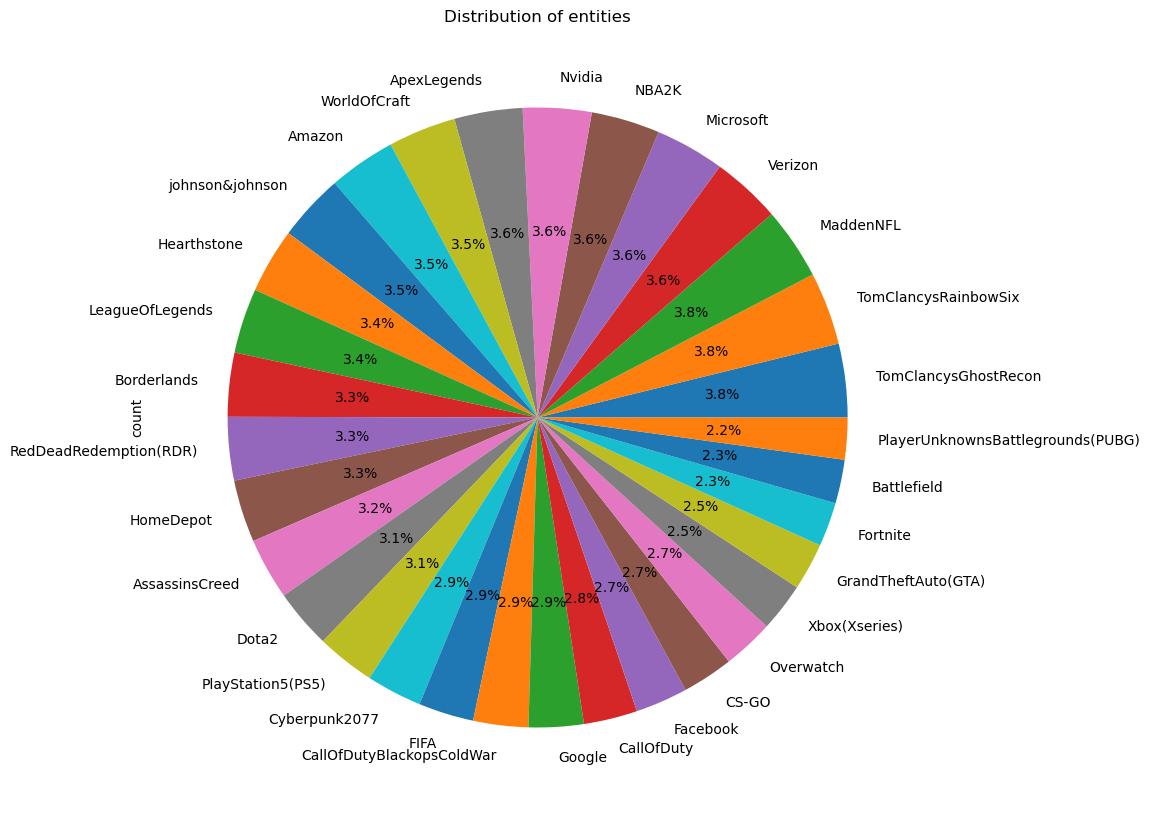
\includegraphics[width=1\linewidth]{images/entity_distribution.png}
    \caption{distribution of entities}
    \label{fig:entity_distribution}
\end{figure}

A pie chart visualizing the frequency of each entity revealed that the entities are relatively uniformly represented, with most entities comprising around 3\% of the dataset each. This near-uniform distribution is beneficial as it suggests that the dataset is not heavily skewed towards a small number of entities, allowing models to learn from a diverse range of subjects.



\subsubsection{Distribution of Sentiment Labels}

The overall distribution of sentiment labels (positive, negative, neutral) was analyzed Fig.\ref{fig:sentiment_distribution}. 

\begin{figure}[H]
    \centering
    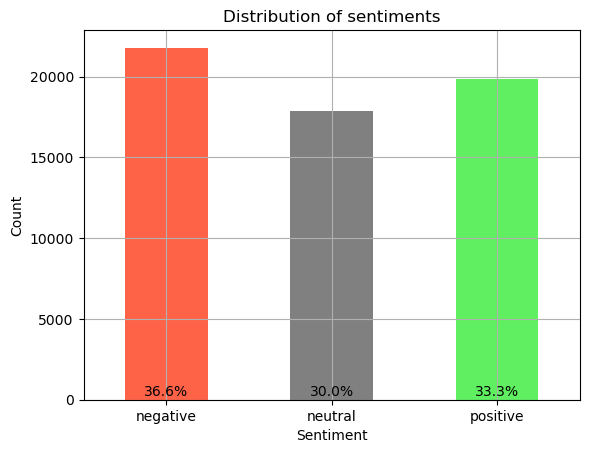
\includegraphics[width=1\linewidth]{images/sentiment_distribution.png}
    \caption{Sentiment Distribution}
    \label{fig:sentiment_distribution}
\end{figure}


A bar chart showed the following approximate distribution:

\begin{itemize}
    \item Negative: Around 36%
    \item Positive: Around 33%
    \item Neutral: Around 30%
\end{itemize}

These proportions indicate that the dataset is reasonably balanced across the three sentiment classes. This balance is crucial for training unbiased models, as it prevents the model from being skewed towards a majority class and helps ensure fair performance evaluation across all sentiments.


\subsubsection{Sentiment Distribution per Entity}

To delve deeper, the sentiment distribution for each individual entity was investigated, Fig.\ref{fig:sentiment_per_entity} 

\begin{figure}[h!]
    \centering
    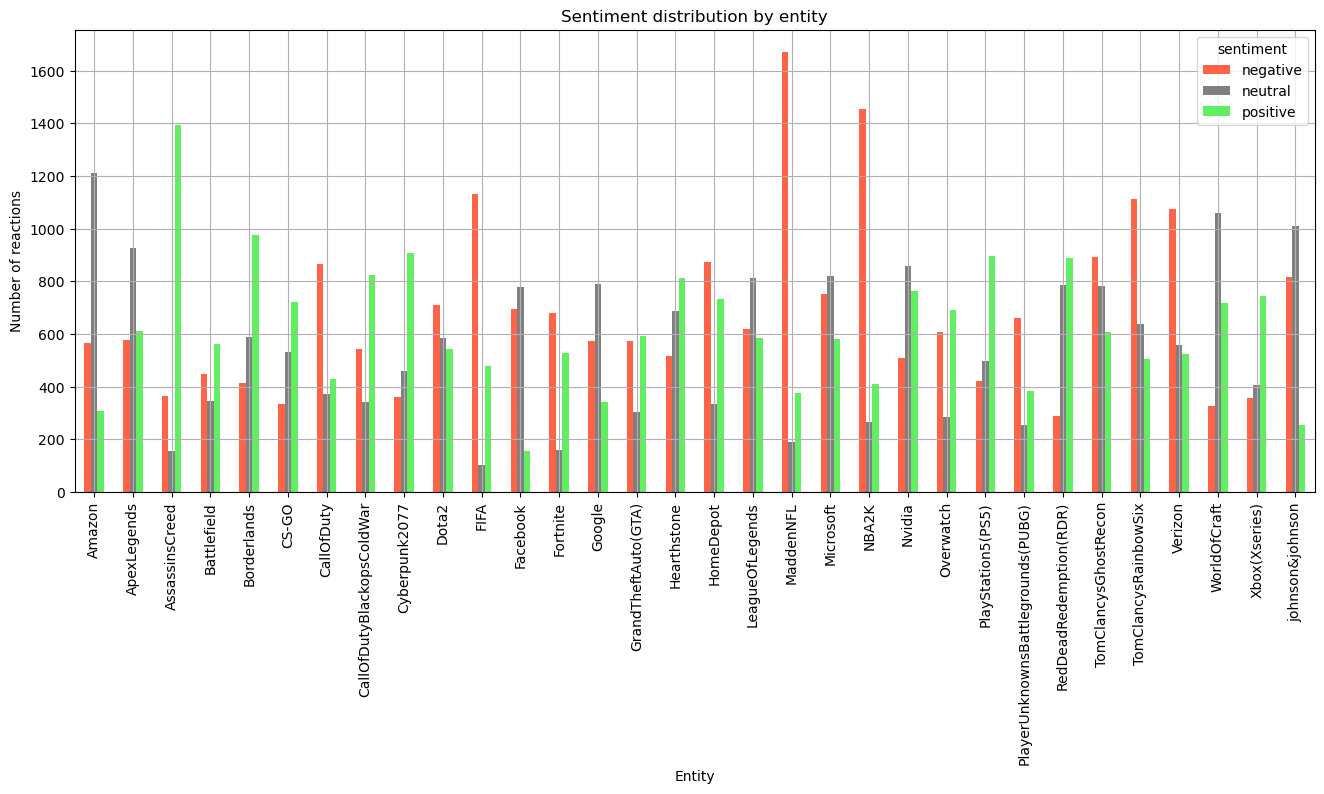
\includegraphics[width=1\linewidth]{images/sentiment_per_entity.png}
    \caption{Sentiment per Entity}
    \label{fig:sentiment_per_entity}
\end{figure}

A grouped bar chart illustrating the number of positive, negative, and neutral reactions for each entity provided valuable insights. For example, it was observed that:
\begin{itemize}
    \item The entity "Madden NFL" tended to have a higher proportion of negative reactions.
    \item "Assassin's Creed" showed a tendency towards more positive reactions.
    \item "Amazon" exhibited a significant number of neutral reactions.
    \item Entities like "Tom Clancy's Ghost Recon" had a more mixed sentiment profile, with comparable numbers of positive, negative, and neutral reactions.
\end{itemize}

This analysis highlights that sentiment can be entity-dependent and showcases the nuanced nature of the dataset. Understanding these entity-specific sentiment patterns is important for interpreting model behavior and identifying potential areas where models might struggle or excel.

\subsection{Text Preprocessing}

Twitter text is inherently noisy, containing slang, abbreviations, URLs, user mentions, hashtags, emojis, and other elements that can hinder the performance of Natural Language Processing (NLP) models. Therefore, a comprehensive text preprocessing was applied to clean and normalize the `tweet\_content` before it was fed into the machine learning and deep learning models.

\begin{enumerate}
    \item Handling Missing Values and Type Conversion: Initially, any `NaN` (Not a Number) entries in the tweet content are converted to empty strings to prevent errors in subsequent processing. The text is then explicitly converted to a string data type.
    \item Removing Web Elements:
     \begin{itemize}
     \item \textbf{URLs}: All HTTP and HTTPS links (e.g., `http://example.com` or `www.example.com`) are removed as they typically do not contribute to the sentiment of the text itself.
     \item \textbf{Mentions}: Twitter mentions (e.g., `@username`) are stripped from the text to remove user-specific addressing.
     \item \textbf{Hashtags}: The '\#' symbol is removed from hashtags, but the textual content of the hashtag is retained (e.g., `\#topic` becomes `topic`), as the hashtag text can often carry sentiment or important keywords.
     \end{itemize}
    \item Character Cleaning and Normalization:
     \begin{itemize}
    \item  \textbf{Emojis and Non-Text Symbols}: Emojis and most other non-text symbols are removed. The process aims to eliminate characters that are not alphanumeric or standard whitespace, while attempting to preserve accented characters common in various languages (e.g., `À-ÿ`) that might be part of valid words.
    \item  \textbf{Numbers}: All numerical digits are deleted from the text.
     \item \textbf{Quotation Marks}: Specific instances of quotation marks (`"`) are removed.
     \item \textbf{Special Characters}: A broader pass removes all characters that are not alphabetical or whitespace (e.g., punctuation, symbols missed in the previous step).
     \item \textbf{Ensure Purely Alphabetic Content}: An additional filter is applied to remove any remaining non-alphabetic characters, further ensuring that only letters and spaces persist before tokenization.
     \end{itemize}
    \item Whitespace Normalization: Multiple whitespace characters (spaces, tabs, newlines) are collapsed into a single space, and any leading or trailing whitespace is removed from the text. This step is applied both during initial cleaning and before tokenization to ensure consistency.
    \item Removing Isolated Single Characters: Single letters surrounded by spaces (e.g., " a ") are removed, as they are often remnants of cleaning or do not carry significant meaning on their own.
    \item Lowercase Conversion: The entire text is converted to lowercase. This ensures uniformity and prevents the model from treating the same word with different capitalization (e.g., "Good" and "good") as distinct tokens.
    \item Tokenization: The cleaned text is then split into individual words or tokens using the `word\_tokenize` function from the NLTK library. Tokenization is a fundamental step in preparing text for NLP models.
    \item Lemmatization: Each token is reduced to its base or dictionary form (lemma) using the `WordNetLemmatizer` from NLTK. For example, "running" would be converted to "run," and "better" might be converted to "good." This helps in consolidating different forms of the same word, reducing the vocabulary size and feature space.
    \item Stop Word Removal: Common English stop words (e.g., "the", "is", "a", "in", "and") are eliminated from the list of tokens using NLTK's predefined `stopwords` list. These words are generally considered to add little semantic value for sentiment classification and can introduce noise.
    \item Filtering Short Tokens: Tokens with a length of three characters or fewer are removed. This step is based on the assumption that very short words (after stop word removal and lemmatization) are less likely to contribute significantly to the overall sentiment.
    \item Retaining Unique Ordered Tokens: Finally, for each tweet, only the unique tokens are retained, and they are kept in the order of their first appearance in the processed tweet.
\end{enumerate}

These preprocessing steps are crucial for transforming the raw, noisy, and unstructured Twitter data into a clean, standardized, and meaningful format. This refined representation is more suitable for the various machine learning and deep learning models employed in this study.
\section{Results}
In this section, we present the results obtained from our sentiment analysis models applied to tweet data. We detail the different approaches and techniques used, focusing on the models that demonstrated effective performance in classifying tweet sentiment.

Initially, we explored traditional Machine Learning (ML) models, such as Support Vector Machines (SVMs), utilizing both Bag-of-Words (BoW) and TF-IDF features for text representation. This established a foundational understanding of model performance on our dataset. Concurrently, we investigated lexicon-based approaches, specifically VADER and TextBlob, to leverage pre-defined sentiment scores.

Subsequently, we delved into various neural network architectures. This included Feedforward Neural Networks (FNNs), Convolutional Neural Networks (CNNs) adapted for text classification, and several Recurrent Neural Networks (RNNs). Within RNNs, we experimented with Long Short-Term Memory (LSTM) networks, Gated Recurrent Units (GRU), and Bidirectional LSTMs (Bi-LSTMs).

Finally, we implemented the powerful transformer-based model, BERT, a state-of-the-art architecture known for its strong performance in natural language processing tasks. Our analysis focused on BERT's ability to accurately classify tweet sentiment.

\subsection{Machine Learning models}

We began our exploration of sentiment analysis by employing traditional Machine Learning (ML) models, specifically Support Vector Machines (SVMs). These models serve as a robust baseline, leveraging established techniques for text classification. To convert raw tweet content into a format understandable by these algorithms, we utilized two distinct feature representation methods: Bag-of-Words (BoW) and TF-IDF (Term Frequency-Inverse Document Frequency). For each SVM variant, we performed meticulous hyperparameter tuning to optimize its performance, ensuring the models were finely tuned for our dataset.

For the hyperparameter optimization of both SVM models, we utilized RandomizedSearchCV. The range of parameters explored and the search configuration are detailed in the table below:

\begin{table}[H]
\centering
\caption{Hyperparameter Tuning Configuration for SVM Models}
\begin{tabular}{|l|l|}
\hline
\multicolumn{2}{|c|}{\textit{SVM Hyperparameters}} \\
\hline
\textbf{Parameter} & \textbf{Values Explored} \\
\hline
C & [0.01, 0.1, 1, 10] \\
kernel & ['linear', 'rbf'] \\
gamma & ['scale', 'auto'] \\
\hline\hline 
\multicolumn{2}{|c|}{\textit{RandomizedSearchCV Settings}} \\
\hline
n\_iter & 5 (number of parameter settings sampled) \\
cv & 3 (number of cross-validation folds) \\
\hline
\end{tabular}
\label{tab:svm_tuning_params}
\end{table}



\subsubsection{\textbf{Support Vector Machines (SVMs) with TF-IDF}}

Our initial SVM approach utilized the TF-IDF Vectorizer to transform the processed tweet texts into numerical features. This method is highly effective for text classification as it weighs words by their frequency within a document, inversely scaled by their frequency across the entire corpus. This approach assigns higher importance to terms that are distinctive to a particular tweet while being less common overall, thus capturing valuable information. The TF-IDF Vectorizer was configured with max\_features=10000, ngram\_range=(1, 2) (allowing for both single words and two-word phrases), min\_df=2 (excluding terms appearing in fewer than two documents), max\_df=0.8 (excluding terms appearing in more than 80\% of documents to remove common words), and incorporated English stop words removal.

Based on the RandomizedSearchCV process, the best parameters identified for the SVM with TF-IDF were 
\begin{itemize}
    \item 'kernel': 'rbf'
    \item 'gamma': 'scale'
    \item 'C': 10
\end{itemize}

The performance of the SVM model with TF-IDF features on the test set is detailed below:

\begin{table}[H]
\centering
\caption{Classification Report for SVM with TF-IDF}
\begin{tabular}{|l|c|c|c|c|}
\hline
\textbf{Class} & \textbf{Precision} & \textbf{Recall} & \textbf{F1-Score} & \textbf{Support} \\
\hline
positive & 0.94 & 0.93 & 0.94 & 4287 \\
negative & 0.94 & 0.92 & 0.93 & 3465 \\
neutral  & 0.90 & 0.94 & 0.92 & 3869 \\
\hline
\textbf{Accuracy} & \multicolumn{4}{|c|}{\textbf{0.93}} \\
\hline
\end{tabular}
\label{tab:svm_tfidf_report}
\end{table}

The SVM with TF-IDF achieved an overall accuracy of 0.93 on the test set, indicating its strong capability in classifying tweet sentiment. The model demonstrated robust performance across all sentiment categories, achieving notably high precision and recall, particularly for the 'positive' class. The F1-scores further underscore a good balance between precision and recall for all classes, confirming the model's effectiveness.

\subsubsection{\textbf{Support Vector Machines (SVMs) with Bag-of-Words}}

We also implemented an SVM model using the Bag-of-Words (BoW) approach with CountVectorizer for text representation. This method converts text into a numerical format by simply counting the occurrences of each word, providing a frequency-based representation of the tweet content. The CountVectorizer was configured with the same parameters as the TF-IDF Vectorizer: max\_features=10000, ngram\_range=(1, 2), min\_df=2, max\_df=0.8, and English stop words removal.

Following the same RandomizedSearchCV process as detailed in Table \ref{tab:svm_tuning_params}, the optimal hyperparameters identified for the SVM with Bag-of-Words were also:
\begin{itemize}
    \item 'kernel': 'rbf'
    \item 'gamma': 'scale'
    \item 'C': 10
\end{itemize}

The model's performance on the test data is detailed in the following table:

\begin{table}[H]
\centering
\caption{Classification Report for SVM with Bag-of-Words}
\begin{tabular}{|l|c|c|c|c|}
\hline
\textbf{Class} & \textbf{Precision} & \textbf{Recall} & \textbf{F1-Score} & \textbf{Support} \\
\hline
positive & 0.92 & 0.91 & 0.91 & 4287 \\
negative & 0.92 & 0.88 & 0.90 & 3465 \\
neutral  & 0.87 & 0.91 & 0.89 & 3869 \\
\hline
\textbf{Accuracy} & \multicolumn{4}{|c|}{\textbf{0.90}} \\
\hline
\end{tabular}
\label{tab:svm_bow_report}
\end{table}


The SVM with Bag-of-Words achieved an accuracy of 0.90, which was slightly lower than the accuracy attained by its TF-IDF counterpart. While still performing well across sentiment classes, particularly for the 'positive' category, the marginal difference in overall accuracy and F1-scores suggests that the TF-IDF representation had a slight advantage in capturing the nuanced importance of words in the dataset.

\subsubsection{\textbf{Comparative Analysis of SVM Models}}

Figure \ref{fig:svm_comparison} provides a visual comparison of the accuracies and confusion matrices for both SVM models, offering a clear overview of their respective performances.

\begin{figure}[h!]
\centering
\begin{subfigure}[t]{0.30\textwidth}
\centering
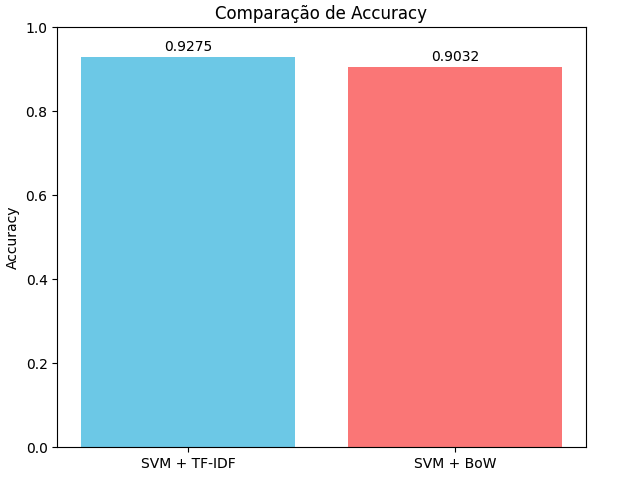
\includegraphics[width=\textwidth]{./images/svm_accuracies.png}
\caption{Accuracy Comparison: SVM + TF-IDF vs. SVM + BoW}
\label{fig:svm_accuracies}
\end{subfigure}
\hfill
\begin{subfigure}[t]{0.30\textwidth}
\centering
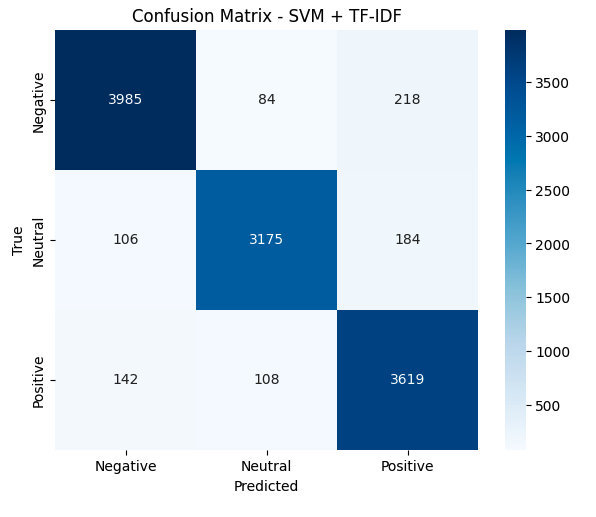
\includegraphics[width=\textwidth]{./images/cm-svm-tfidf.png}
\caption{Confusion Matrix - SVM + TF-IDF}
\label{fig:cm_tfidf}
\end{subfigure}
\hfill
\begin{subfigure}[t]{0.30\textwidth}
\centering
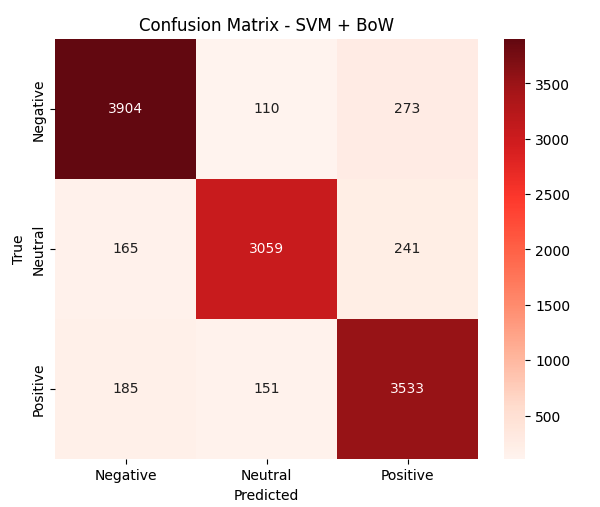
\includegraphics[width=\textwidth]{./images/cm-svm-bow.png}
\caption{Confusion Matrix - SVM + BoW}
\label{fig:cm_bow}
\end{subfigure}
\caption{Performance Comparison of SVM Models}
\label{fig:svm_comparison}
\end{figure}

The comparative accuracy bar chart clearly illustrates that TF-IDF features generally yielded superior performance for SVM in this sentiment classification task. The confusion matrices offer a detailed view of the models' classification strengths and weaknesses across the different sentiment classes. Both models exhibited a tendency to misclassify some 'neutral' tweets, which often present greater ambiguity in sentiment compared to clearly 'positive' or 'negative' content. However, we can see in the confusion matrix that TF-IDF model indicates slightly better classification rates across all categories.

These traditional ML models establish a solid baseline for our sentiment analysis efforts, demonstrating the effectiveness of classic text representation techniques when paired with a powerful classifier like SVM. Their performance underscores the enduring importance of careful feature engineering in achieving robust machine learning outcomes.




\subsection{ Traditional approaches}

Beyond machine learning models, we explored lexicon-based approaches for sentiment analysis. These methods rely on predefined dictionaries of words, each associated with a sentiment score. We specifically utilized TextBlob and VADER (Valence Aware Dictionary and sEntiment Reasoner),


\subsubsection{ \textbf{TextBlob Sentiment Analysis}}

TextBlob is a Python library for processing textual data, providing a simple API for common natural language processing (NLP) tasks, including sentiment analysis. Its sentiment analysis model returns two properties: polarity (a float ranging from -1.0 to 1.0, where -1 is negative, 0 is neutral, and 1 is positive) and subjectivity (a float ranging from 0.0 to 1.0, where 0.0 is very objective and 1.0 is very subjective).

For sentiment classification, we defined a rule-based approach:
\begin{itemize}
    \item Polarity greater than 0.1 was classified as 'Positive'.
    \item Polarity less than -0.1 was classified as 'Negative'.
    \item Polarity between -0.1 and 0.1 (inclusive) was classified as 'Neutral'.
\end{itemize}

The performance of TextBlob on the validation dataset, using this classification logic, is summarized below:

\begin{table}[H]
\centering
\caption{Classification Report for TextBlob (Validation Set)}
\begin{tabular}{|l|c|c|c|c|}
\hline
\textbf{Class} & \textbf{Precision} & \textbf{Recall} & \textbf{F1-Score} & \textbf{Support} \\
\hline
Negative & 0.53 & 0.44 & 0.48 & 266 \\
Neutral  & 0.39 & 0.39 & 0.39 & 285 \\
Positive & 0.53 & 0.61 & 0.57 & 276 \\
\hline
\textbf{Accuracy} & \multicolumn{4}{|c|}{\textbf{0.48}} \\
\hline
\end{tabular}
\label{tab:textblob_validation_report}
\end{table}

TextBlob achieved an accuracy of 0.48 on the validation set. While it performed reasonably well for 'Positive' sentiment, its ability to correctly identify 'Neutral' and 'Negative' tweets was limited, as indicated by lower precision and recall scores for those categories. This suggests that its lexicon-based rules might struggle with the nuances and informal language often found in tweets.

\begin{figure}[H]
    \centering
    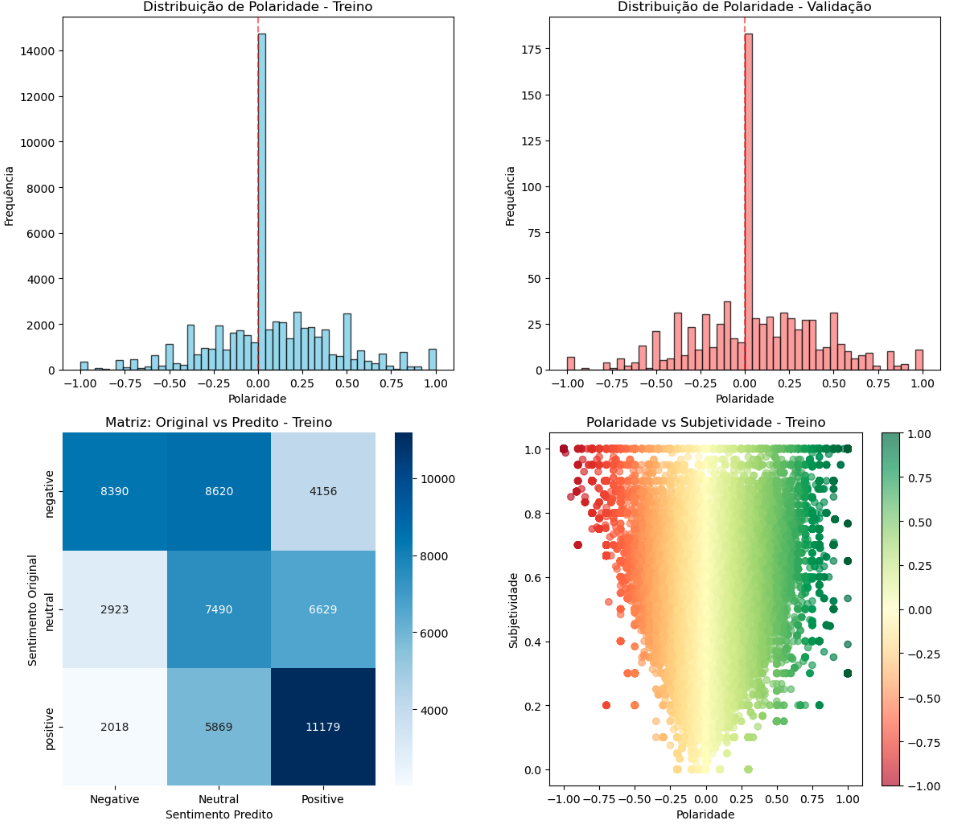
\includegraphics[width=1\linewidth]{images/text-blob.png}
    \caption{Correlation Matrix and Polarity Distribution}
    \label{fig:enter-label}
\end{figure}

The polarity distributions show a concentration of scores around zero, indicating many tweets are classified as neutral. The confusion matrix highlights challenges in distinguishing between sentiment classes, particularly the 'Neutral' class, which is often misclassified.


\subsubsection{ \textbf{VADER Sentiment Analysis}}
VADER (Valence Aware Dictionary and sEntiment Reasoner) is a lexicon and rule-based sentiment analysis tool specifically attuned to sentiments expressed in social media contexts. Unlike TextBlob's polarity, VADER provides a compound score (normalized between -1 and 1) representing the overall sentiment intensity, along with positive, negative, and neutral scores. Its strength lies in recognizing common linguistic features of internet language, such as capitalization, exclamation marks, and emojis, which significantly influence sentiment.

For classification, we used VADER's compound score with a standard threshold:
\begin{itemize}
    \item Compound score >= 0.05: 'Positive'
    \item Compound score <= -0.05: 'Negative'
    \item Compound score between -0.05 and 0.05: 'Neutral'
\end{itemize}

The performance of VADER on the validation dataset is presented below:

\begin{table}[H]
\centering
\caption{Classification Report for VADER (Training Set)}
\begin{tabular}{|l|c|c|c|c|}
\hline
\textbf{Class} & \textbf{Precision} & \textbf{Recall} & \textbf{F1-Score} & \textbf{Support} \\
\hline
Negative & 0.56 & 0.58 & 0.57 & 21166 \\
Neutral  & 0.34 & 0.18 & 0.24 & 17042 \\
Positive & 0.50 & 0.68 & 0.57 & 19066 \\
\hline
\textbf{Accuracy} & \multicolumn{4}{|c|}{\textbf{0.50}} \\
\hline
\end{tabular}
\label{tab:vader_training_report}
\end{table}


VADER outperformed TextBlob, achieving an accuracy of 0.50 on the validation set. Its higher precision, recall, and F1-scores across all classes, especially for 'Negative' and 'Positive' sentiments, highlight its effectiveness in handling the specific characteristics of social media text. The 'Neutral' class still presented some challenges, but VADER's performance was better than TextBlob.

Figure \ref{fig:vader_analysis} provides a visual representation of VADER's sentiment scores and classifications:

\begin{figure}[H]
    \centering
    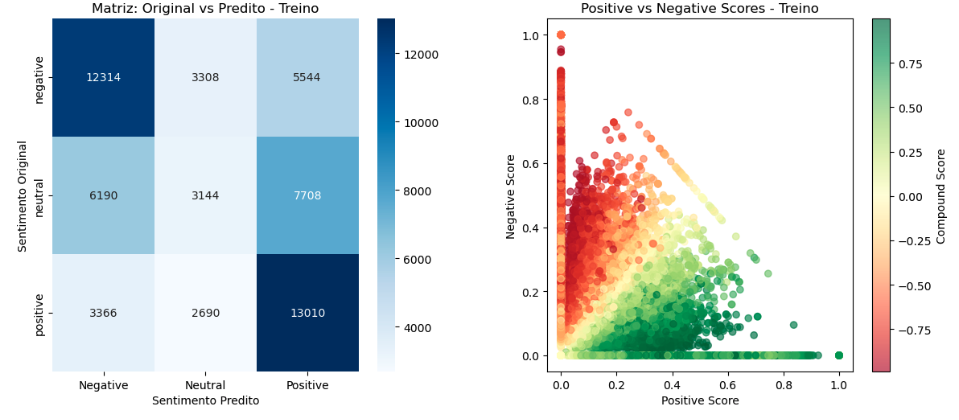
\includegraphics[width=1\linewidth]{images/vader.png}
    \caption{Correlation Matrix, Positive vs Negative}
    \label{fig:vader_analysis}
\end{figure}

The compound score distributions show a clearer separation of positive and negative sentiments compared to TextBlob. The confusion matrix further demonstrates VADER's improved classification abilities, but the neutral class still has problems.


\subsubsection{\textbf{Comparative Analysis}}

Comparing TextBlob and VADER, it's clear that VADER provides a more robust and accurate sentiment analysis for tweets among the lexicon-based methods. 

However, when comparing these traditional lexicon-based approaches to the Machine Learning models (SVMs) previously discussed, it is evident that the SVMs achieved significantly higher overall accuracies.  These results demonstrate that while lexicon-based models offer fast and lightweight sentiment scoring without explicit training, their performance is generally surpassed by supervised machine learning models that can learn complex patterns directly from the labeled data. This difference highlights the benefit of data-driven learning in capturing intricate semantic and contextual relationships, which static lexicons may struggle to interpret.



\subsection{Deep Learning Models}

After explored traditional machine learning and lexicon-based approaches, we explore into Deep Learning (DL) models to leverage their capability in learning complex patterns directly from raw data. This section details our experiments with Feedforward Neural Networks (FNNs), Convolutional Neural Networks (CNNs) adapted for text, Recurrent Neural Networks (RNNs), and the transformer-based BERT model.

\subsubsection{\textbf{Feedforward Neural Networks (FNNs)}}

Our initial deep learning experiments began with Feedforward Neural Networks (FNNs). These models consist of multiple layers where information flows in one direction, from input to output, without cycles. FNNs are a foundational architecture for learning complex, non-linear relationships. We integrated an Embedding layer as the first component, which maps words to dense vector representations, allowing the model to capture semantic similarities between words. We explored two main configurations for our FNNs:

\textbf{First FNN Architecture
}

The first FNN architecture used a straightforward approach to flatten the output of the embedding layer before feeding it into dense layers. This creates a single, long feature vector from the word embeddings.

The model's architecture is as follows:

\begin{itemize}
    \item Embedding Layer: Maps vocabulary words to 100-dimensional dense vectors.
    \item Flatten Layer: Converts the 2D output of the embedding layer into a 1D vector.
    \item Dense Layer (128 units): Fully connected layer with ReLU activation.
    \item Dropout Layer (0.5): Regularization to prevent overfitting by randomly setting 50\% of input units to 0.
    \item Dense Layer (64 units): Another fully connected layer with ReLU activation.
    \item Dropout Layer (0.3): Regularization, setting 30\% of input units to 0.
    \item Output Layer (3 units): Dense layer with Softmax activation for multiclass classification (positive, neutral, negative).
\end{itemize}

The model was compiled using the Adam optimizer with a learning rate of 0.001 and categorical crossentropy as the loss function.

\textbf{Second FNN Architecture}

The second FNN architecture aimed to improve upon the first by replacing the Flatten layer with GlobalAveragePooling1D and incorporating BatchNormalization and L2 regularization into the dense layers. GlobalAveragePooling1D reduces the dimensionality by averaging embedding vectors across the sequence length, preserving more semantic information than flattening. BatchNormalization helps stabilize and accelerate training, while L2 regularization penalizes large weights, which can mitigate overfitting.

The model's architecture is as follows:

\begin{itemize}
    \item Embedding Layer: Maps vocabulary words to 100-dimensional dense vectors.
    \item GlobalAveragePooling1D Layer: Averages the word embeddings across the sequence.
    \item Dense Layer (128 units): Fully connected layer with ReLU activation and L2 regularization (0.01).
    \item BatchNormalization Layer: Normalizes the activations of the previous layer.
    \item Dropout Layer (0.5): Regularization.
    \item Dense Layer (64 units): Another fully connected layer with ReLU activation and L2 regularization (0.01).
    \item BatchNormalization Layer: Normalizes the activations.
    \item Dropout Layer (0.5): Regularization.
    \item Output Layer (3 units): Dense layer with Softmax activation.
    \item 
\end{itemize}
This model was also compiled using the Adam optimizer with a learning rate of 0.001, categorical crossentropy loss.

\textbf{Performance of FNN Models
}

Across both FNN architectures, while the models showed promising learning curves on the training data, they consistently exhibited signs of overfitting. The training accuracy would increase steadily, and the training loss would decrease, but the validation accuracy often plateaued or even declined after a few epochs, accompanied by an increase in validation loss. This indicates that the models were memorizing the training data rather than generalizing well to unseen examples. This behavior is a common challenge with FNNs on text data, as they may struggle to capture local features or sequences without more specialized architectures like CNNs or RNNs.

The subsequent figures illustrate this overfitting behavior:

\begin{figure}[h!]
\centering

% Primeira linha: FNN Architecture 1 Accuracy and Loss
\begin{subfigure}[t]{0.48\textwidth}
\centering
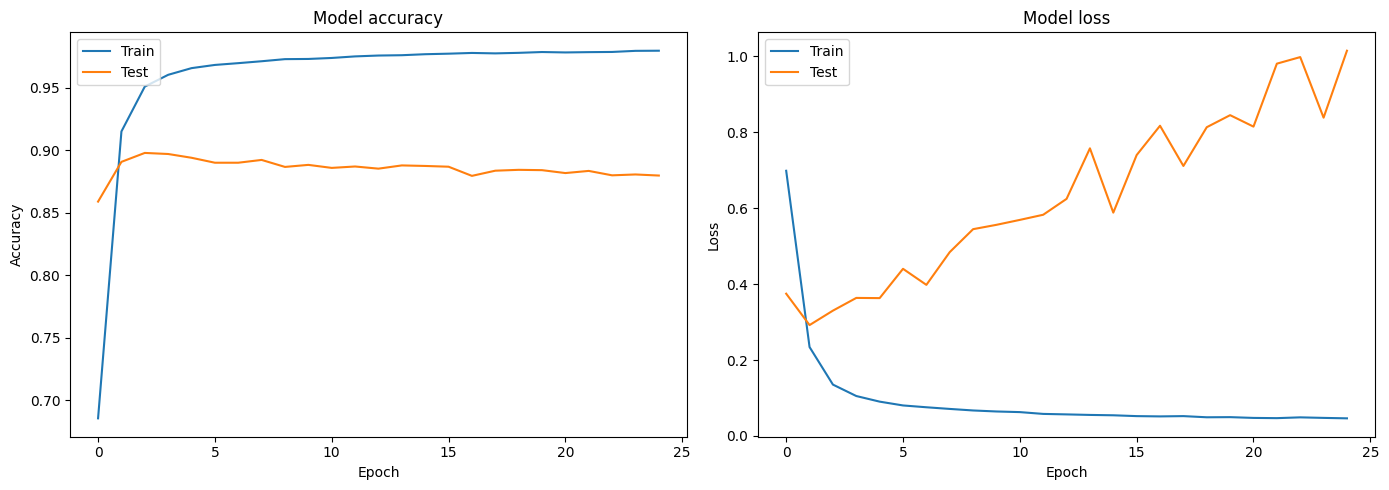
\includegraphics[width=\textwidth]{./images/fnn1-acc.png}
\caption{FNN Architecture 1: Train vs Validation Accuracy and Loss}
\label{fig:fnn1_accuracy}
\end{subfigure}

\vspace{0.5cm} % Espaçamento vertical entre as linhas

% Segunda linha: FNN Architecture 2 Accuracy and Loss
\begin{subfigure}[t]{0.48\textwidth}
\centering
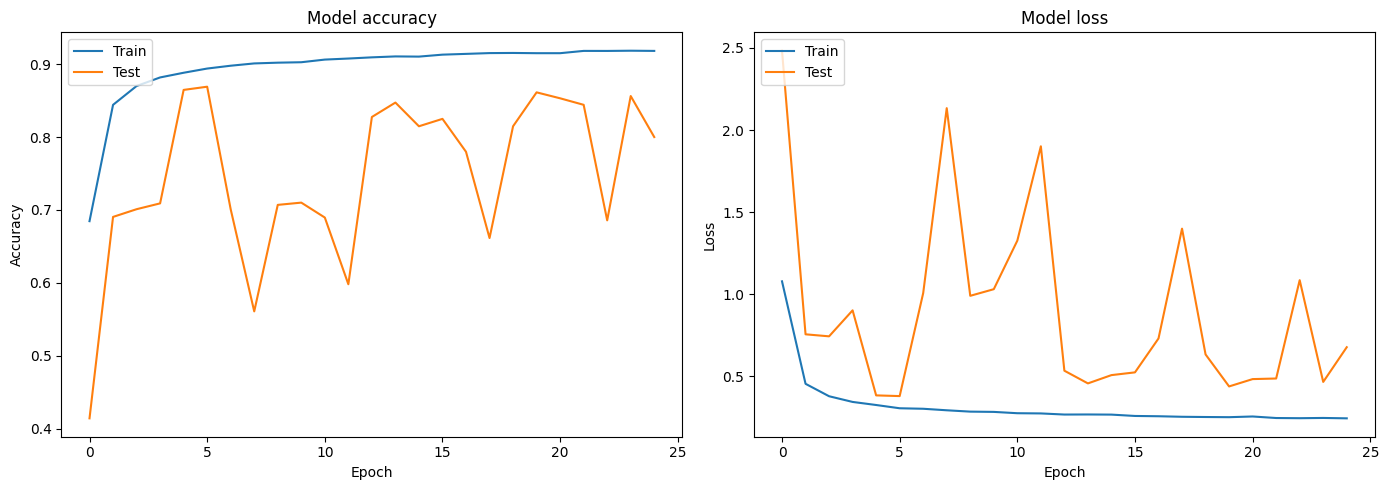
\includegraphics[width=\textwidth]{./images/fnn2-acc.png}
\caption{FNN Architecture 2: Train vs Validation Accuracy and Loss}
\label{fig:fnn1_loss}
\end{subfigure}

\vspace{0.5cm}

% Terceira linha: Confusion Matrices lado a lado
\begin{subfigure}[t]{0.23\textwidth}
\centering
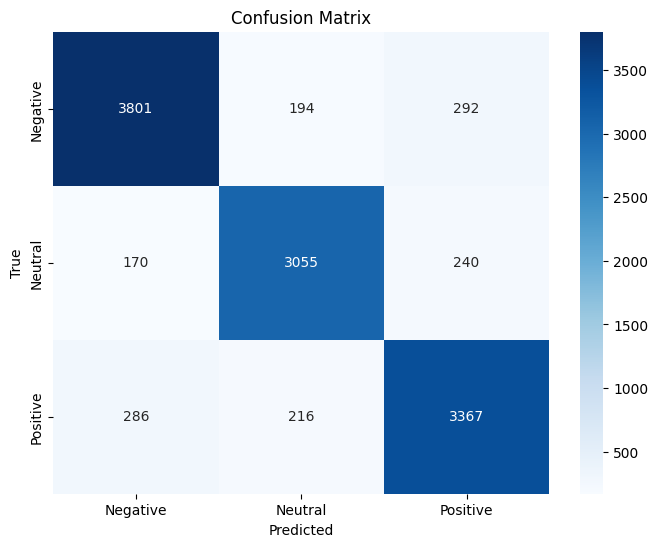
\includegraphics[width=\textwidth]{./images/fnn1-cm.png}
\caption{FNN Architecture 1: Confusion Matrix}
\label{fig:fnn2_accuracy}
\end{subfigure}
\hfill
\begin{subfigure}[t]{0.23\textwidth}
\centering
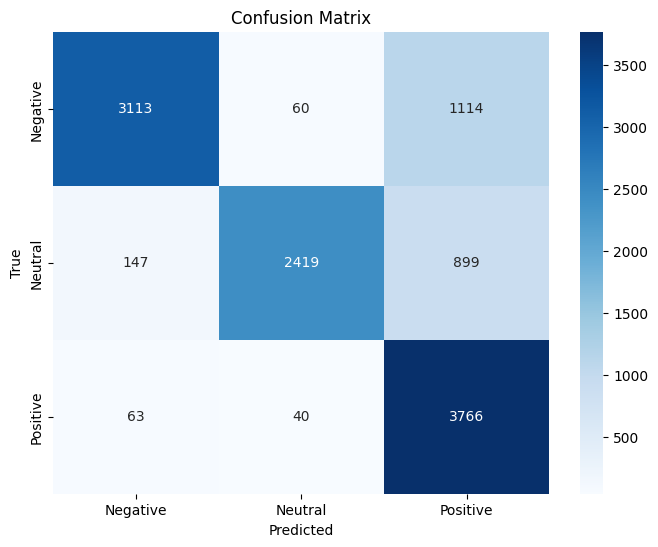
\includegraphics[width=\textwidth]{./images/fnn2-cm.png}
\caption{FNN Architecture 2: Confusion Matrix}
\label{fig:fnn2_loss}
\end{subfigure}
\caption{Training and Validation Performance of FNN Models}
\label{fig:fnn_performance}
\end{figure}

Given these limitations, particularly the persistent overfitting, we proceeded to explore more specialized deep learning architectures better suited for sequential data like text.

\subsubsection{\textbf{Convolutional Neural Networks (CNNs)}}

Following our experiments with FNNs, we moved on to Convolutional Neural Networks (CNNs). While traditionally known for image processing, CNNs have proven effective for text classification. They excel at capturing local patterns (like n-grams) through convolutional filters, regardless of their position in the sequence, and then aggregating these features.

We implemented two distinct CNN architectures:

\textbf{First CNN Architecture}

Our first CNN model utilized a single Conv1D layer followed by GlobalMaxPooling1D. This design aims to identify the most salient feature (the highest value detected by a filter) across the entire sequence for each filter.

The model's architecture is as follows:

\begin{itemize}
    \item Embedding Layer: Maps vocabulary words to 100-dimensional dense vectors (vocab\_size input dimension, maxlen input length).
    \item Conv1D Layer (128 filters): Applies 1D convolution with a kernel\_size of 5, using ReLU activation to detect local patterns.
    \item GlobalMaxPooling1D Layer: Extracts the maximum value from each feature map, effectively capturing the most important feature detected by each filter.
    \item Dense Layer (64 units): Fully connected layer with ReLU activation and L2 regularization (0.01).
    \item Dropout Layer (0.5): Regularization.
    \item Output Layer (3 units): Dense layer with Softmax activation for multiclass classification.
\end{itemize}

The model was compiled using the Adam optimizer with a learning rate of 0.001 and categorical crossentropy as the loss function.

\begin{figure}[h!]
    \centering
    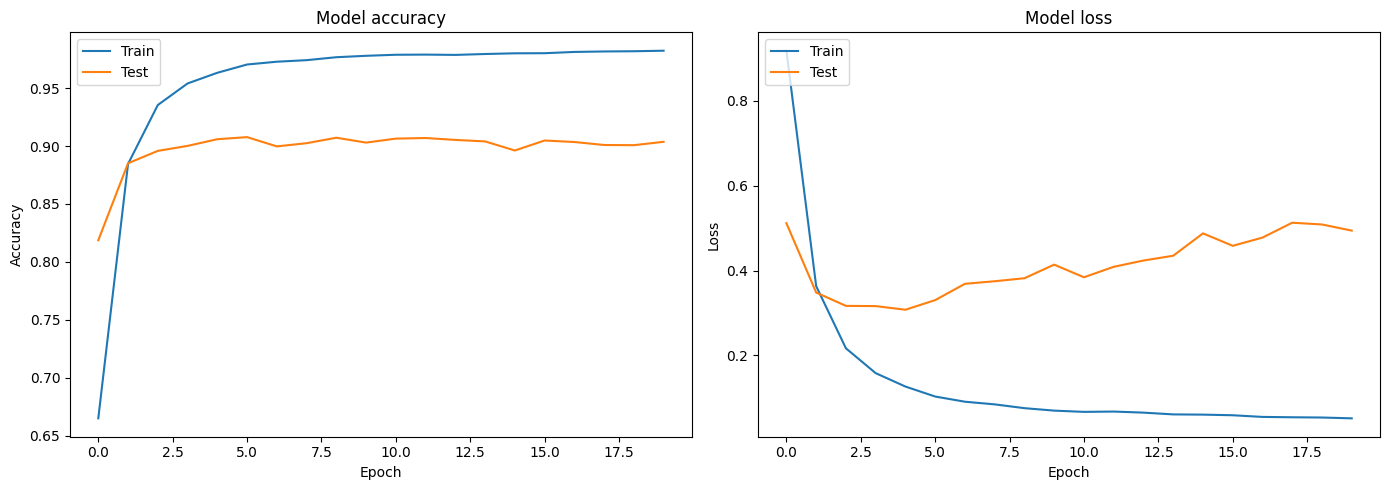
\includegraphics[width=1\linewidth]{images/cnn1-acc.png}
\caption{CNN Architecture 1: Train vs Validation Accuracy and Loss}
    \label{fig:cnn-acc-1}
\end{figure}

Similar to the FNNs, this first CNN architecture, despite its convolutional capabilities, still displayed significant overfitting. While it learned to classify the training data very well, its performance on the validation set would often diverge, indicating a struggle to generalize to new, unseen tweets. This suggests that a single-filter approach, even with regularization, might not be sufficient to capture the diverse patterns needed for robust sentiment classification on this dataset. The  figure \ref{fig:cnn-acc-1} illustrate the training and validation performance, clearly showing overfitting.

\textbf{Second CNN Architecture}

To address the limitations of the single-filter approach and improve generalization, our second CNN architecture adopted a multi-filter strategy, processing different n-gram sizes (3, 4, and 5) in parallel. This allows the model to extract a richer set of local features from the text, capturing patterns of varying lengths simultaneously. The outputs from these parallel filters are then concatenated and passed through a denser network.

The model's architecture is as follows:

\begin{itemize}
    \item Input Layer: Defines the input sequence length (maxlen).
    \item Embedding Layer: Maps vocabulary words to 100-dimensional dense vectors.
    \item Parallel Conv1D Layers (64 filters each):
     \begin{itemize}
 \item Conv1D with kernel\_size=3, ReLU activation, and L2 regularization (0.01).
     \item Conv1D with kernel\_size=4, ReLU activation, and L2 regularization (0.01).
     \item Conv1D with kernel\_size=5, ReLU activation, and L2 regularization (0.01).
     \end{itemize}
    \item Parallel GlobalMaxPooling1D Layers: Extracts the maximum feature from each of the three convolutional outputs.
    \item Concatenate Layer: Combines the outputs from the three pooling layers into a single vector.
    \item Dense Layer (32 units): Fully connected layer with ReLU activation and L2 regularization (0.05).
    \item Dropout Layer (0.6): Regularization.
    \item Output Layer (3 units): Dense layer with Softmax activation.
\end{itemize}

This model was compiled using the Adam optimizer with a learning rate of 0.001, categorical crossentropy loss.

\begin{figure}[h!]
\centering
\begin{subfigure}[t]{0.48\textwidth}
\centering
% Replace with your actual CNN 2 Accuracy plot
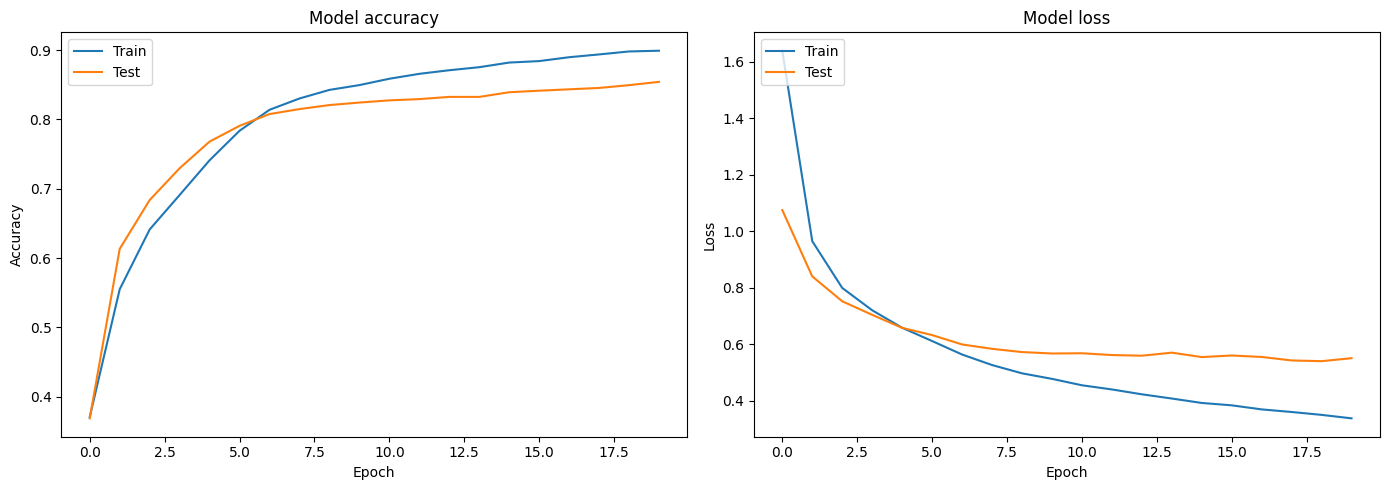
\includegraphics[width=\textwidth]{./images/cnn2-acc.png}
\caption{CNN Architecture 2: Train vs Validation Accuracy and Loss}
\label{fig:cnn2_accuracy}
\end{subfigure}
\hfill
\begin{subfigure}[t]{0.30\textwidth}
\centering
% Replace with your actual CNN 2 Loss plot
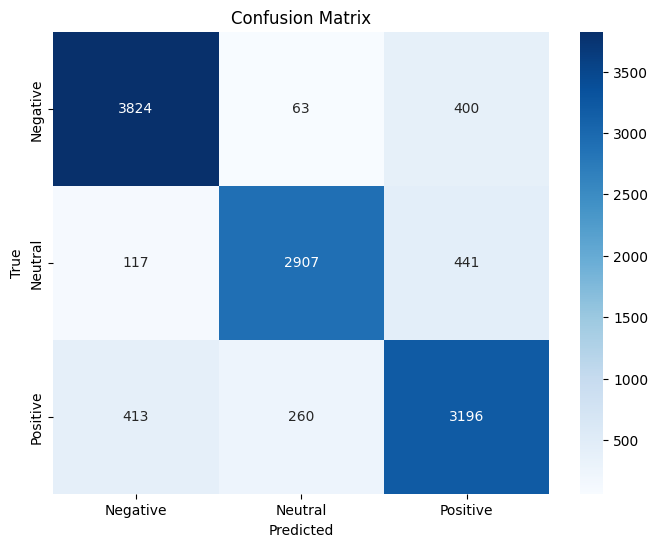
\includegraphics[width=\textwidth]{./images/cnn-cm.png}
\caption{CNN Architecture 2: CNN Confusion Matrix}
\label{fig:cnn2_loss}
\end{subfigure}
\caption{Training and Validation Performance of CNN Architecture 2}
\label{fig:cnn2_performance}
\end{figure}

This multi-filter CNN architecture showed significantly improved performance compared to the first CNN and the FNN models. It achieved a notably higher accuracy on the validation set, indicating better generalization capabilities due to its ability to extract diverse local patterns.

\begin{table}[H]
\centering
\caption{Classification Report for CNN Architecture 2 (Test Set)}
\begin{tabular}{|l|c|c|c|c|}
\hline
\textbf{Class} & \textbf{Precision} & \textbf{Recall} & \textbf{F1-Score} & \textbf{Support} \\
\hline
negative & 0.88 & 0.89 & 0.89 & 4287 \\
neutral  & 0.90 & 0.84 & 0.87 & 3465 \\
positive & 0.79 & 0.83 & 0.81 & 3869 \\
\hline
\textbf{Accuracy} & \multicolumn{4}{|c|}{\textbf{0.85}} \\
\hline
\end{tabular}
\label{tab:cnn2_classification_report}
\end{table}

This model achieved an accuracy of 0.85, demonstrating its effectiveness. The high precision and recall for 'negative' and 'neutral' classes are particularly good, though 'positive' sentiment shows a slightly lower precision.

However, even with these improvements, the training curves still indicate a slight degree of overfitting, Fig. \ref{fig:cnn2_loss}. While less pronounced than in the FNNs or the first CNN, the validation loss might still begin to rise slightly, or the validation accuracy might plateau while training accuracy continues to improve. This suggests that while the architecture is better suited for text, further regularization or more complex models might yield even better generalization.

Despite this minor overfitting, the second CNN architecture stands as a strong performer, achieving comparable results to our best SVM model and demonstrating the potential of CNNs for text classification tasks. Next we explore Recurrent Neural Networks to capture sequential dependencies in text.


\subsubsection{\textbf{Recurrent Neural Networks (RNNs)}}

Moving beyond models that primarily capture local features (like CNNs) or disregard sequence entirely (like FNNs), we implemented Recurrent Neural Networks (RNNs). RNNs are specifically designed to process sequential data, making them ideal for text. They maintain an internal state that allows them to remember information from previous steps in the sequence, which is crucial for understanding context and dependencies in sentences. We focused on two prominent RNN architectures: Long Short-Term Memory (LSTM) and Gated Recurrent Units (GRU).

\textbf{First LSTM Architecture: Simple LSTM}

Our initial RNN experiment utilized a basic Long Short-Term Memory (LSTM) layer. LSTMs are a type of RNN capable of learning long-term dependencies, addressing the vanishing gradient problem inherent in simpler RNNs.

The model's architecture is as follows:

\begin{itemize}
    \item Embedding Layer: Maps vocabulary words to 64-dimensional dense vectors, with maxlen input length.
    \item LSTM Layer (64 units): The core LSTM layer processing the sequence.
    \item Output Layer (3 units): Dense layer with Softmax activation for multiclass classification.
\end{itemize}

The model was compiled using categorical crossentropy loss and the Adam optimizer.

\begin{figure}[h!]
    \centering
    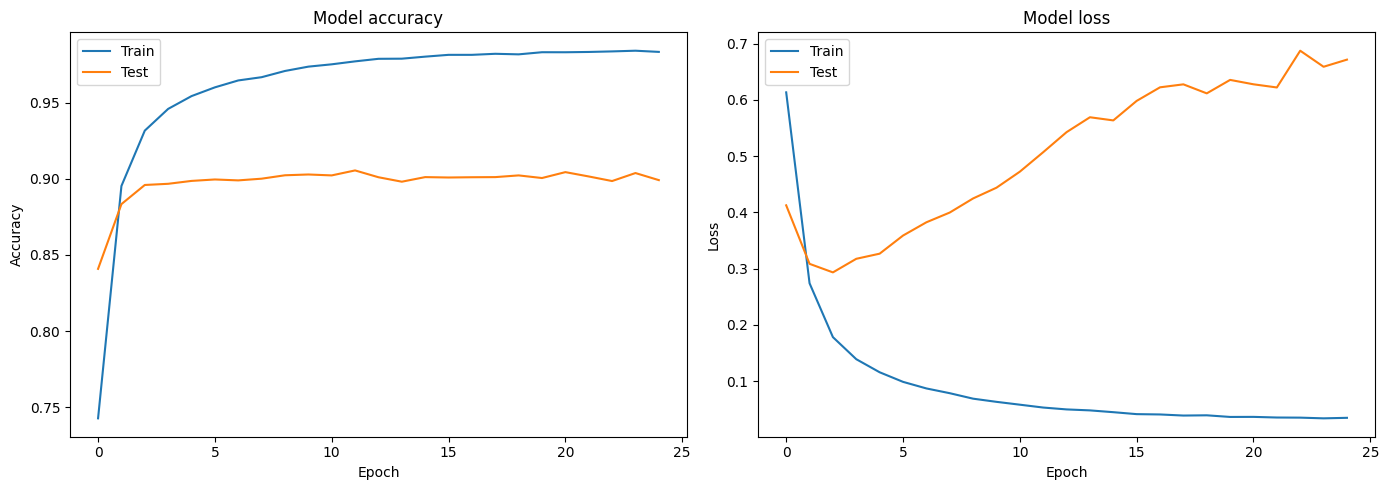
\includegraphics[width=1\linewidth]{images/lstm1.png}
    \caption{Simple LSTM Architecture: Train vs Validation Accuracy and Loss}
    \label{fig:enter-label}
\end{figure}

This basic LSTM model, despite its capability for sequential data, exhibited significant overfitting. While it learned to perform very well on the training data, its performance on the validation set quickly plateaued or even deteriorated. This suggests that the simple architecture lacked sufficient regularization or complexity to generalize effectively to unseen text.

\textbf{Second LSTM Architecture}

To combat the overfitting observed in the simple LSTM and further enhance performance, we developed a more complex LSTM architecture incorporating several regularization techniques.

The model's architecture is as follows:
\begin{itemize}
    \item Input Layer: Defines the input sequence shape (maxlen).
    \item Embedding Layer: Maps vocabulary words to a higher dimension (D=128), with mask\_zero=True to correctly handle padding.
    \item SpatialDropout1D Layer (0.8): Applies dropout to the entire feature map of the embedding, promoting independence between features.
    \item LSTM Layer (64 units): Processes the sequence, with dropout=0.3, recurrent\_dropout=0.3 (for regularization within the recurrent connections), return\_sequences=True (to pass output to the next layer if stacked LSTMs were used, though here it feeds into GlobalMaxPooling), and kernel\_regularizer=l2(0.01).
    \item GlobalMaxPooling1D Layer: Extracts the most salient feature from the LSTM output sequence.
    \item Dense Layer (64 units): Fully connected layer with ReLU activation and L2 regularization (0.001).
    \item BatchNormalization Layer: Normalizes activations.
    \item Dropout Layer (0.5): Regularization.
    \item Dense Layer (32 units): Another fully connected layer with ReLU activation.
    \item BatchNormalization Layer: Normalizes activations.
    \item Dropout Layer (0.5): Regularization.
    \item Output Layer (3 units): Dense layer with Softmax activation.
\end{itemize}

The model was compiled using the Adam optimizer with a learning rate of 0.001, categorical crossentropy loss.

\begin{figure}[h!]
\centering
\begin{subfigure}[t]{0.48\textwidth}
\centering
% Replace with your actual CNN 2 Accuracy plot
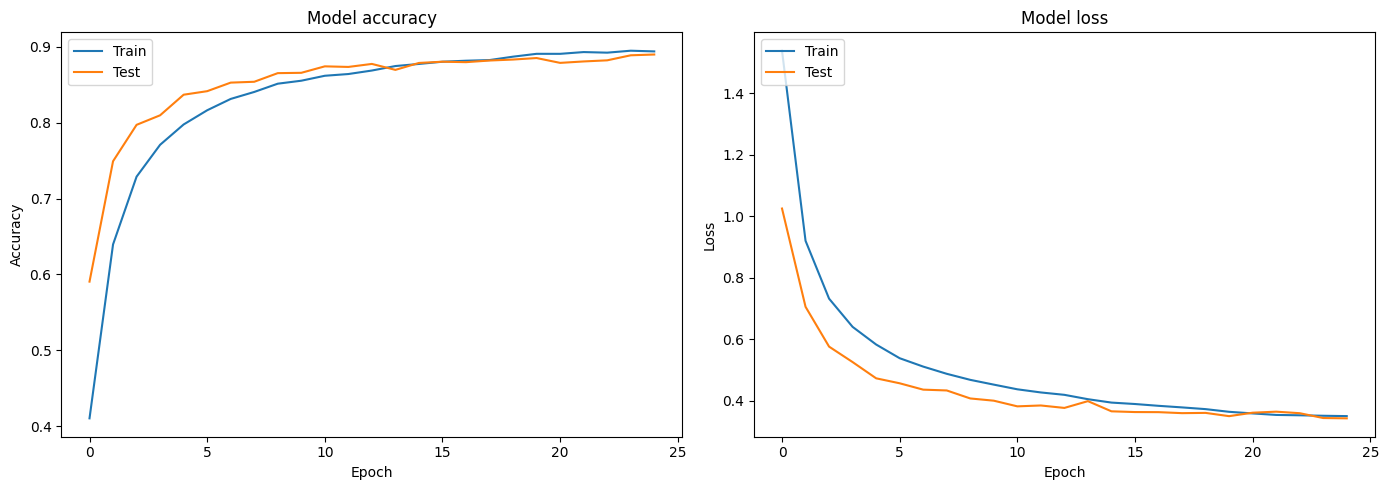
\includegraphics[width=\textwidth]{./images/lstm-acc.png}
\caption{LSTM Architecture 2: Train vs Validation Accuracy and Loss}
\label{fig:cnn2_ac1curacy}
\end{subfigure}
\hfill
\begin{subfigure}[t]{0.30\textwidth}
\centering
% Replace with your actual CNN 2 Loss plot
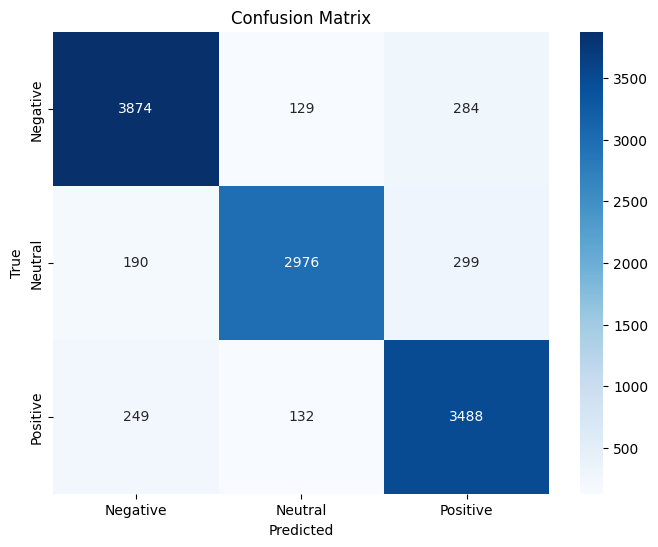
\includegraphics[width=\textwidth]{./images/lstm-cm.png}
\caption{LSTM Architecture 2: Confusion Matrix}
\label{fig:cnn2_lo1ss}
\end{subfigure}
\caption{Training and Validation Performance of LSTM Architecture 2}
\label{fig:cnn2_pe1rformance}
\end{figure}

This improved LSTM architecture demonstrated excellent performance on the test set, achieving a high accuracy and well-balanced precision, recall, and F1-scores across all sentiment classes. The various regularization techniques (SpatialDropout, recurrent dropout, L2 regularization, BatchNormalization, and Dropout) significantly reduced overfitting, leading to much better generalization.

\begin{table}[H]
\centering
\caption{Classification Report for Improved LSTM (Test Set)}
\begin{tabular}{|l|c|c|c|c|}
\hline
\textbf{Class} & \textbf{Precision} & \textbf{Recall} & \textbf{F1-Score} & \textbf{Support} \\
\hline
negative & 0.90 & 0.90 & 0.90 & 4287 \\
neutral  & 0.92 & 0.86 & 0.89 & 3465 \\
positive & 0.86 & 0.90 & 0.88 & 3869 \\
\hline
\textbf{Accuracy} & \multicolumn{4}{|c|}{\textbf{0.89}} \\
\hline
\end{tabular}
\label{tab:lstm2_classification_report}
\end{table}

This LSTM model achieved a remarkable overall accuracy of 0.89, marking it as one of the best-performing models thus far. Its ability to correctly classify 'neutral' tweets with high precision is particularly noteworthy.

\textbf{GRU Architecture: Gated Recurrent Unit
}

In parallel to the improved LSTM, we also developed a model based on Gated Recurrent Units (GRUs). GRUs are a slightly simplified variant of LSTMs, often offering comparable performance with fewer parameters, which can lead to faster training. Like LSTMs, they are designed to handle sequential data and mitigate the vanishing gradient problem.

The GRU model's architecture closely mirrors that of the improved LSTM, incorporating similar regularization strategies:

\begin{itemize}
    \item Input Layer: Defines the input sequence shape (maxlen).
    \item Embedding Layer: Maps vocabulary words to a higher dimension (D=128), with mask\_zero=True.
    \item SpatialDropout1D Layer (0.8): Applies dropout to the embedding feature map.
    \item GRU Layer (64 units): Processes the sequence, with dropout=0.3, recurrent\_dropout=0.3, return\_sequences=True, and kernel\_regularizer=l2(0.01).
    \item GlobalMaxPooling1D Layer: Extracts the most salient feature from the GRU output.
    \item Dense Layer (64 units): Fully connected layer with ReLU activation and L2 regularization (0.001).
    \item BatchNormalization Layer: Normalizes activations.
    \item Dropout Layer (0.5): Regularization.
    \item Dense Layer (32 units): Another fully connected layer with ReLU activation.
    \item BatchNormalization Layer: Normalizes activations.
    \item Dropout Layer (0.5): Regularization.
    \item Output Layer (3 units): Dense layer with Softmax activation.
\end{itemize}

The model was compiled using the Adam optimizer with a learning rate of 0.001, categorical crossentropy loss.

\begin{figure}[h!]
\centering
\begin{subfigure}[t]{0.48\textwidth}
\centering
% Replace with your actual CNN 2 Accuracy plot
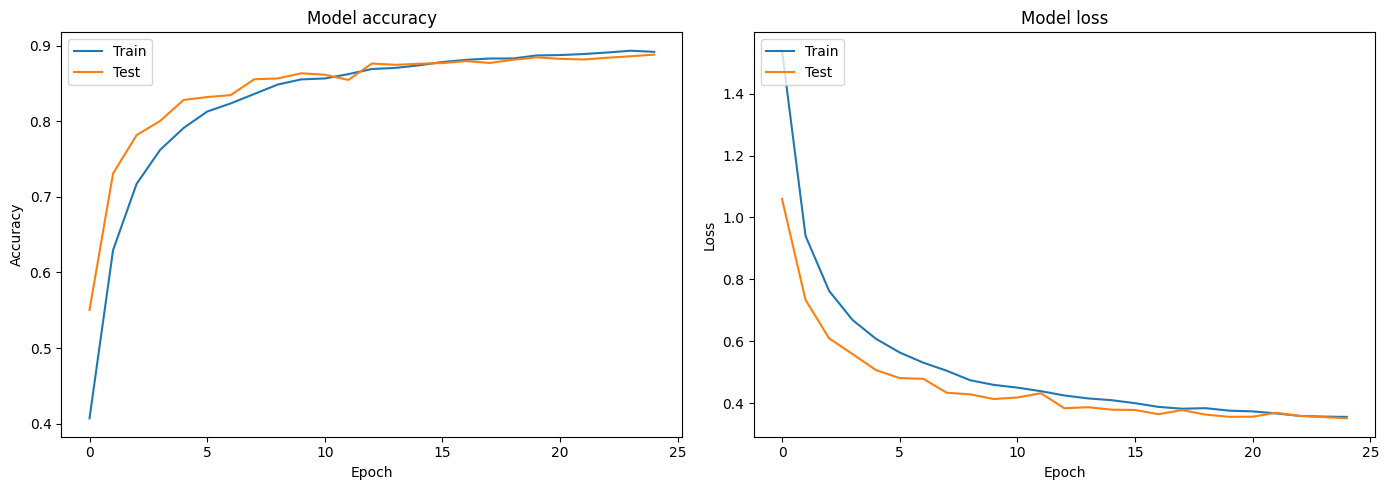
\includegraphics[width=\textwidth]{./images/gru-acc.png}
\caption{GRU Architecture: Train vs Validation Accuracy and Loss}
\label{fig:cnn22_accuracy}
\end{subfigure}
\hfill
\begin{subfigure}[t]{0.30\textwidth}
\centering
% Replace with your actual CNN 2 Loss plot
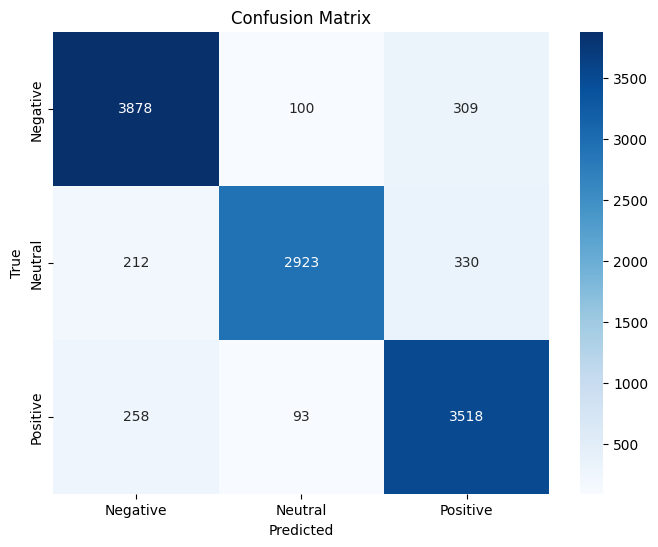
\includegraphics[width=\textwidth]{./images/gru-cm.png}
\caption{GRU Architecture: Confusion Matrix}
\label{fig:cnn24_loss}
\end{subfigure}
\caption{Training and Validation Performance of GRU Architecture}
\label{fig:cnn22_performance}
\end{figure}

The GRU model also yielded strong results on the test set, achieving an accuracy comparable to the improved LSTM. It demonstrated excellent precision and recall across all classes, showcasing its effectiveness in capturing sequential dependencies for sentiment analysis.

\begin{table}[H]
\centering
\caption{Classification Report for GRU Model (Test Set)}
\begin{tabular}{|l|c|c|c|c|}
\hline
\textbf{Class} & \textbf{Precision} & \textbf{Recall} & \textbf{F1-Score} & \textbf{Support} \\
\hline
negative & 0.89 & 0.90 & 0.90 & 4287 \\
neutral  & 0.94 & 0.84 & 0.89 & 3465 \\
positive & 0.85 & 0.91 & 0.88 & 3869 \\
\hline
\textbf{Accuracy} & \multicolumn{4}{|c|}{\textbf{0.89}} \\

\hline
\end{tabular}
\label{tab:gru_classification_report}
\end{table}

The GRU model achieved an overall accuracy of 0.89, matching the performance of the improved LSTM. It shows particularly high precision for the 'neutral' class and strong recall for 'negative' and 'positive' sentiments.

The similar high accuracy and balanced F1-scores between the improved LSTM and GRU models indicate that both architectures, when properly regularized and configured, are highly effective for sequential text classification tasks. Their ability to handle long-term dependencies and capture contextual information makes them superior to FNNs for this type of data, and their performance is on par with the best CNN model.

\textbf{Bidirectional LSTM (Bi-LSTM)}

In addition to the standard LSTM and GRU architectures, we also explored Bidirectional LSTMs (Bi-LSTMs). Bi-LSTMs enhance the ability of recurrent networks to understand context by processing the input sequence in both forward and backward directions independently, and then concatenating their outputs. This allows the model to capture dependencies from both past and future contexts, which can be particularly beneficial for tasks like sentiment analysis where the meaning of a word can be influenced by words that appear later in the sentence.

\begin{figure}[h!]
\centering
\begin{subfigure}[t]{0.48\textwidth}
\centering
% Replace with your actual CNN 2 Accuracy plot
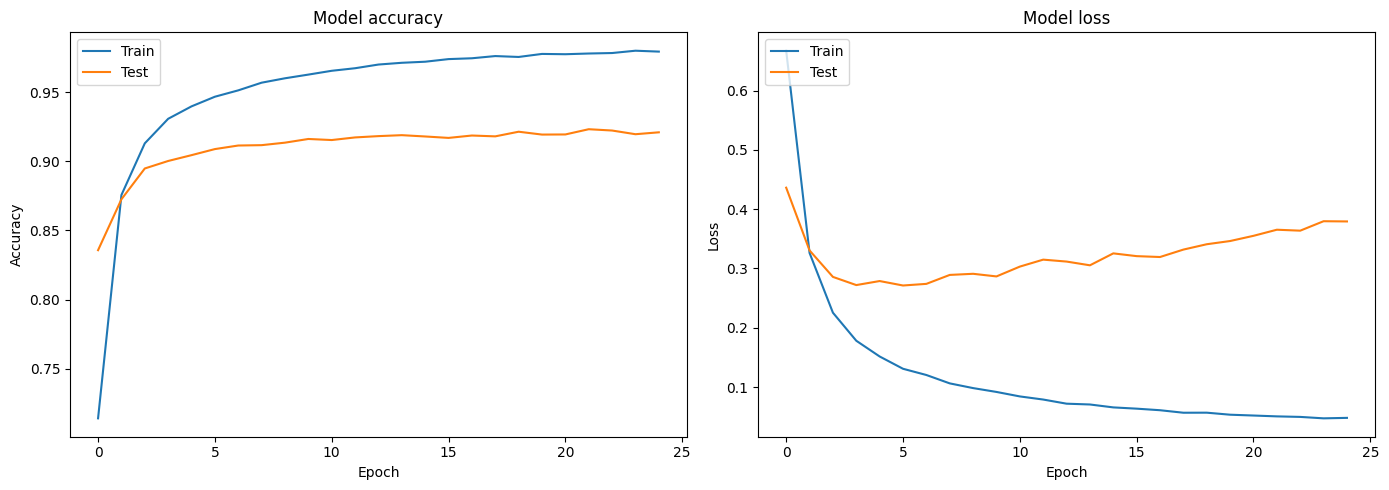
\includegraphics[width=\textwidth]{./images/bi1.png}
\caption{Bi-LSTM Architecture 1: Train vs Validation Accuracy and Loss}
\label{fig:cnn2_ac12curacy}
\end{subfigure}
\hfill
\begin{subfigure}[t]{0.48\textwidth}
\centering
% Replace with your actual CNN 2 Loss plot
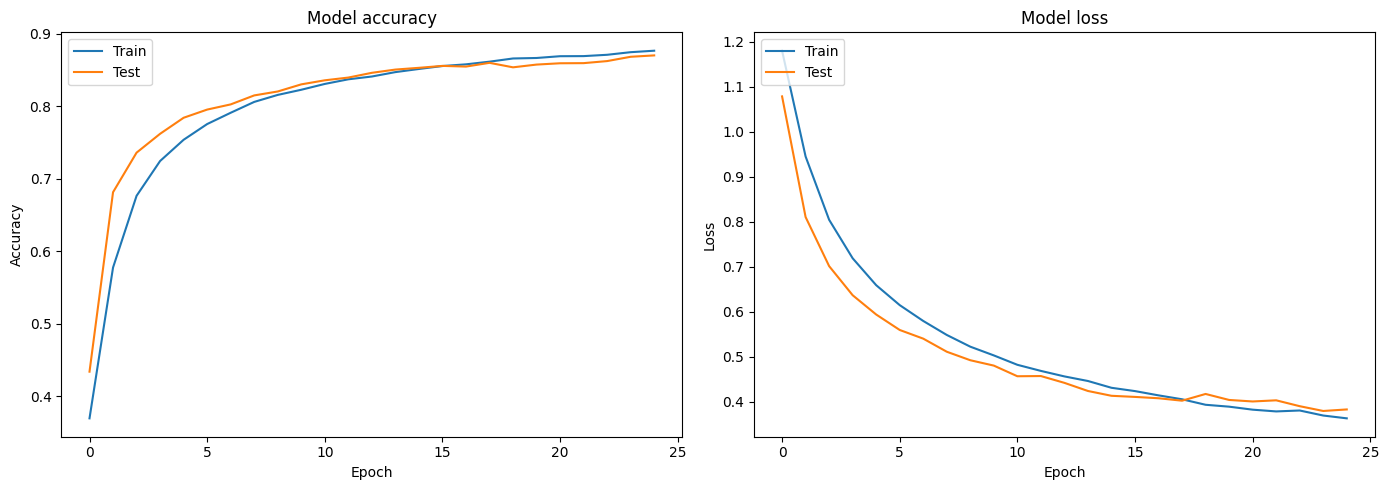
\includegraphics[width=\textwidth]{./images/bi2.png}
\caption{Bi-LSTM Architecture 2: Train vs Validation Accuracy and Loss}
\label{fig:cnn2_lo23ss}
\end{subfigure}
\caption{Training and Validation Performance of Bi-LSTM Architecture}
\label{fig:cnn2_2performance}
\end{figure}
\begin{table}[H]
\centering
\caption{Classification Report for Bi-LSTM Architecture 2 (Test Set)}
\begin{tabular}{|l|c|c|c|c|}
\hline
\textbf{Class} & \textbf{Precision} & \textbf{Recall} & \textbf{F1-Score} & \textbf{Support} \\
\hline
negative & 0.85 & 0.91 & 0.88 & 4285 \\
neutral  & 0.93 & 0.81 & 0.86 & 3507 \\
positive & 0.85 & 0.88 & 0.87 & 3829 \\
\hline
\textbf{Accuracy} & \multicolumn{4}{|c|}{\textbf{0.87}} \\
\hline
\end{tabular}
\label{tab:classification_report_modelo}
\end{table}

Similar to our other recurrent network experiments, our initial simple Bi-LSTM model exhibited significant overfitting, indicating that a basic configuration was insufficient to generalize effectively to unseen data. However, through the implementation of a second, more advanced Bi-LSTM architecture incorporating similar regularization techniques (such as SpatialDropout1D, recurrent dropout, and L2 regularization) as our improved LSTM and GRU models, we achieved similarly strong results. This improved Bi-LSTM model demonstrated excellent performance, effectively capturing the sequential nuances of the social media text and yielding high accuracy and well-balanced precision, recall, and F1-scores across all sentiment classes, aligning closely with the high-performing improved LSTM and GRU models.

\subsection{Transformer-based Models: BERT}

Finally, we tried into Transformer-based models, specifically BERT (Bidirectional Encoder Representations from Transformers). BERT models revolutionized Natural Language Processing (NLP) by pre-training deep bidirectional representations from unlabeled text, enabling them to understand context from both left and right sides of a word. This pre-training on massive datasets allows them to capture highly sophisticated linguistic patterns, making them incredibly powerful for various downstream tasks like sentiment analysis, typically through a process called fine-tuning.

\subsubsection{\textbf{Pre-trained BERT Model (cardiffnlp/twitter-roberta-base-sentiment)}}

Our initial approach involved directly utilizing a pre-trained BERT model specifically fine-tuned for sentiment analysis on Twitter data: cardiffnlp/twitter-roberta-base-sentiment \cite{camacho-collados-etal-2022-tweetnlp}. This model, a RoBERTa variant, is already optimized for social media text characteristics. We loaded its tokenizer and the pre-trained classification model and evaluated its performance on our dataset.

\begin{table}[H]
\centering
\caption{Classification Report for Pre-trained BERT (cardiffnlp/twitter-roberta-base-sentiment)}
\begin{tabular}{|l|c|c|c|c|}
\hline
\textbf{Class} & \textbf{Precision} & \textbf{Recall} & \textbf{F1-Score} & \textbf{Support} \\
\hline
negative & 0.68 & 0.76 & 0.72 & 21432 \\
neutral & 0.49 & 0.40 & 0.44 & 17327 \\
positive & 0.66 & 0.69 & 0.67 & 19342 \\
\hline
\textbf{Accuracy} & \multicolumn{4}{|c|}{\textbf{0.63}} \\
\hline
\end{tabular}
\label{tab:pretrained_bert_report}
\end{table}

While this pre-trained model provided a baseline, its overall accuracy of 0.6286 was not as high as anticipated, especially when compared to our better-performing CNN and RNN models. The F1-score for the 'neutral' class was particularly low, indicating that while it was trained on Twitter data, it might not perfectly align with the specific distribution or nuances of sentiment in our dataset. This suggested that a custom fine-tuning approach would be more beneficial.



\subsubsection{\textbf{BERT Fine-tuning for Sentiment Classification}}

Given the limitations of the directly applied pre-trained model, we proceeded with fine-tuning a BERT model on our specific dataset. Fine-tuning involves continuing the training of a pre-trained model on a smaller, task-specific dataset, allowing it to adapt its learned representations to the new task while retaining its general language understanding.

The fine-tuned BERT model achieved superior results compared to all previous models, demonstrating the power of transfer learning from large-scale pre-trained transformers.

\begin{table}[H]
\centering
\caption{Classification Report for Fine-tuned BERT (Test Set)}
\begin{tabular}{|l|c|c|c|c|}
\hline
\textbf{Class} & \textbf{Precision} & \textbf{Recall} & \textbf{F1-Score} & \textbf{Support} \\
\hline
negative & 0.92 & 0.93 & 0.93 & 4287 \\
neutral  & 0.93 & 0.92 & 0.92 & 3465 \\
positive & 0.92 & 0.92 & 0.92 & 3869 \\
\hline
\textbf{Accuracy} & \multicolumn{4}{|c|}{\textbf{0.93}} \\
\hline
\end{tabular}
\label{tab:fine_tuned_bert_report}
\end{table}

The fine-tuned BERT model achieved an impressive overall accuracy of 0.93, making it the highest-performing model in our entire evaluation. It demonstrated consistently high precision, recall, and F1-scores across all three sentiment classes, indicating robust and balanced classification performance.

\begin{figure}[h!]
\centering
\begin{subfigure}[t]{0.48\textwidth}
\centering
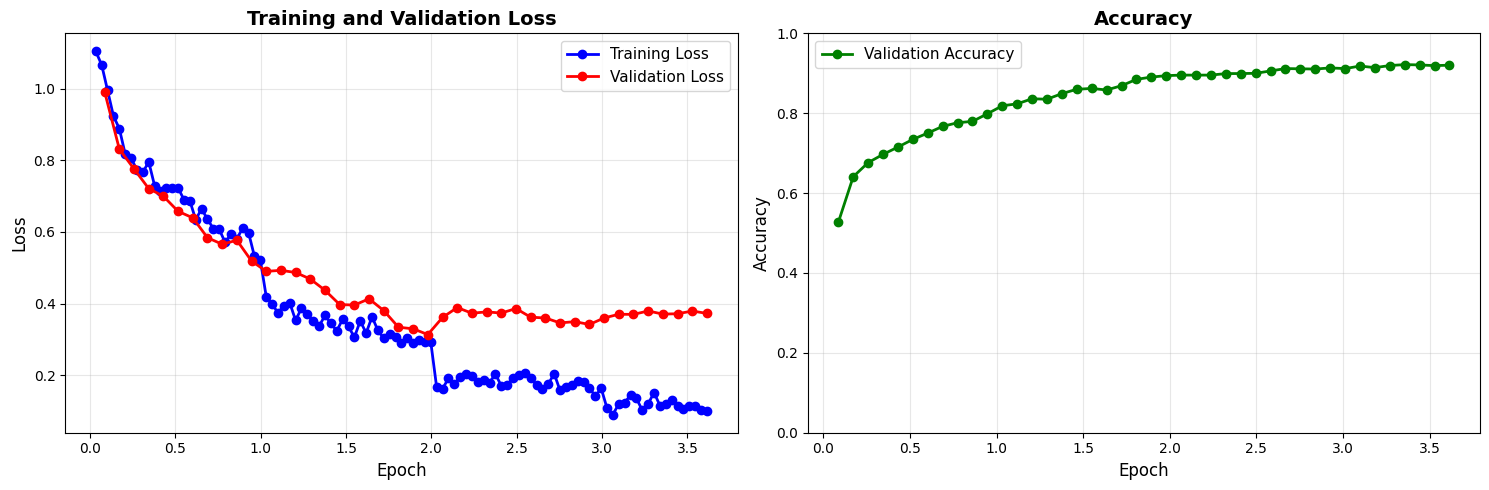
\includegraphics[width=\textwidth]{./images/bert.png}
\caption{Fine-tuned BERT: Training and Validation Loss and Accuracy}
\label{fig:bert_loss}
\end{subfigure}
\hfill
\begin{subfigure}[t]{0.48\textwidth}
\centering
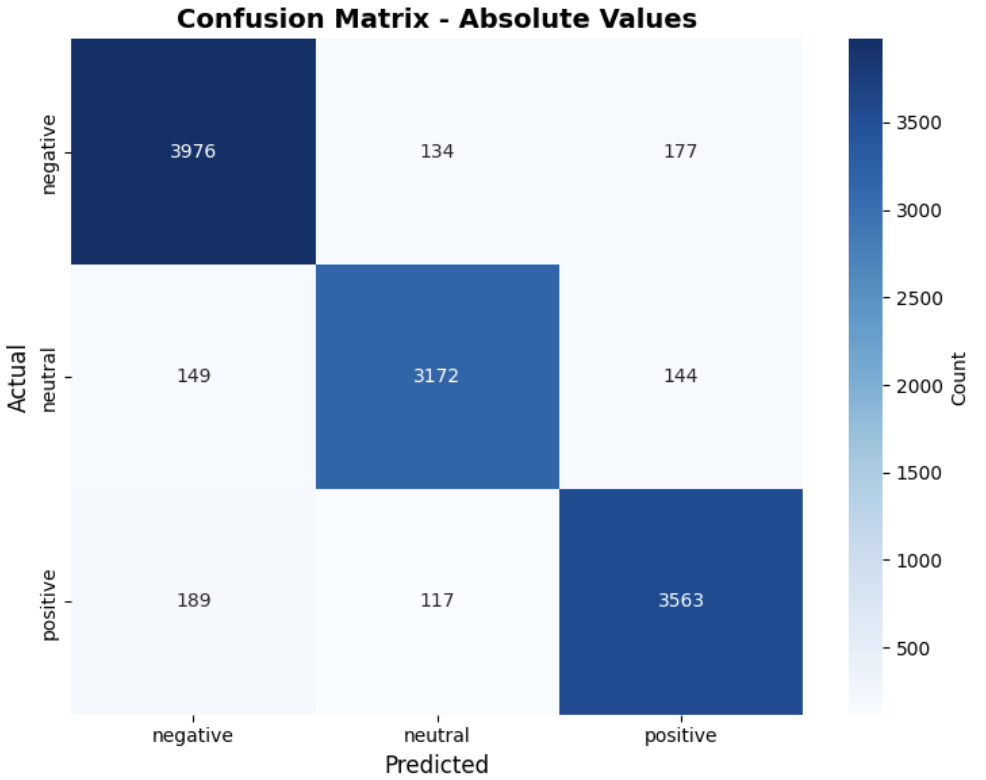
\includegraphics[width=0.4\textwidth]{./images/bert-cm.png}
\caption{Fine-tuned BERT: Confusion Matrix}
\label{fig:bert_accuracy}
\end{subfigure}
\caption{Training and Validation Performance of Fine-tuned BERT Model}
\label{fig:bert_performance}
\end{figure}

The per-class analysis also highlights the model's balanced performance:
\begin{itemize}
\item Negative: Accuracy=0.93, Count=4287
\item Neutral: Accuracy=0.92, Count=3465
\item Positive: Accuracy=0.92, Count=3869
\end{itemize}

\subsubsection{\textbf{Computational Considerations}}

It is important to note that while BERT models deliver state-of-the-art performance, they are significantly more computationally intensive than the traditional machine learning models (SVMs) and even the simpler deep learning architectures (FNNs, CNNs, RNNs). Training the BERT model, even with fine-tuning, required substantial computational resources and took approximately 4 to 5 hours to complete on our setup. This computational cost is a crucial factor to consider when deploying such models, especially in resource-constrained environments or for real-time applications.

Despite the higher computational demands, the fine-tuned BERT model consistently yielded the best performance across all experiments, affirming its position as a leading approach for complex NLP tasks like sentiment analysis on social media text. Our further experiments with various parameters consistently confirmed BERT's superior results.








\section{Comparison with State-of-the-Art Methods}

To thoroughly evaluate the effectiveness of our developed models for sentiment analysis on Twitter data, we compared their performance against relevant state-of-the-art approaches found in academic literature. This comparison helps contextualize our findings, highlighting the strengths and limitations of various methodologies in handling the complexities of social media text. Our analysis includes a review of studies employing traditional machine learning, deep learning architectures, and modern transformer-based models specifically applied to sentiment analysis on Twitter or similar short text datasets.

\begin{enumerate}
\item \textbf{Machine Learning for Depression Detection on Twitter}: In the study \textit{Learning with Support Vector Machine for Depression Detection on Twitter} \cite{costa2021image}, the authors investigated the application of machine learning for classifying depressive and non-depressive posts on Twitter. Using a dataset of over 31,000 tweets, their findings demonstrated that a Support Vector Machine (SVM) model achieved an accuracy of 94\%, along with 91\% precision, recall, and F1-score. This study provides a strong benchmark for traditional machine learning methods on Twitter data, particularly concerning binary classification tasks.

\item \textbf{Systematic Comparison of CNN and RNN for NLP}: The paper \textit{A Systematic Comparison of Convolutional Neural Networks and Recurrent Neural Networks for Text Classification} \cite{zhou2017systematic} presents a comprehensive analysis of CNNs and RNNs across various Natural Language Processing (NLP) tasks, including sentiment classification. This work highlights the general strengths of these deep learning architectures: CNNs excel at extracting position-invariant local features, and RNNs are adept at modeling sequential dependencies. 

\item \textbf{Review of Sentiment Analysis on Twitter using NLP Models}: The paper \textit{Sentiment Analysis of Twitter data using NLP Models: A Comprehensive Review} \cite{prabhakar2024sentiment} is a recent and comprehensive review that surveys various approaches and methodologies for Twitter sentiment analysis. It synthesizes findings from multiple studies, discussing machine learning, deep learning, and hybrid models, while particularly emphasizing the emergence and impact of transformer-based architectures like BERT and GPT. This review provides valuable context on current trends, key models, and the importance of pre-processing and feature extraction in achieving effective sentiment analysis on Twitter data, presenting a broad spectrum of reported results.
\end{enumerate}

After analyzing these external works, we compiled a comparative summary of our models' performance alongside relevant benchmarks from the literature.

\begin{table}[H]
\centering
\caption{Performance Metrics of Our Developed Models on Test Set}
\begin{tabular}{||c|c|c|c|c||}
\hline
\textbf{Model Type} & \textbf{Accuracy} & \textbf{Precision} & \textbf{Recall} & \textbf{F1-Score} \\
\hline \hline
SVM with TF-IDF & \textbf{0.93} & \textbf{0.93} & \textbf{0.93} & \textbf{0.93} \\
\hline
CNN (Multi-Filter) & 0.85 & 0.86 & 0.85 & 0.85 \\
\hline
Improved LSTM & 0.89 & 0.89 & 0.89 & 0.89 \\
\hline
GRU & 0.89 & 0.89 & 0.89 & 0.89 \\
\hline
Bi-LSTM & 0.87 & 0.88 & 0.87 & 0.86 \\
\hline
BERT (Pre-trained) & 0.62 & 0.61 & 0.62 & 0.62 \\
\hline
BERT (Fine-tuned) & \textbf{0.93} & \textbf{0.93} & \textbf{0.93} & \textbf{0.93} \\
\hline
\end{tabular}
\label{tab:our_models_results}
\end{table}

\begin{table}[H]
\centering
\caption{Performance for Depression Detection}
\begin{tabular}{||l|c|c|l||}
\hline
\textbf{Model / Study} & \textbf{Metric} & \textbf{Score} & \textbf{Notes} \\
\hline \hline
SVM~\cite{costa2021image} & Accuracy & 0.94 & Binary classification \\
\hline
CNN~\cite{zhou2017systematic} & Accuracy & 82.38 & Sentiment Analyses \\
GRU~\cite{zhou2017systematic} & Accuracy & 86.32 & Sentiment Analyses \\
LSTM~\cite{zhou2017systematic} & Accuracy & 84.51 & Sentiment Analyses \\
\hline
BERT~\cite{prabhakar2024sentiment} & Accuracy & 0.93 & Comparative review \\
BERT~\cite{prabhakar2024sentiment} & Accuracy & 0.89 & Comparative review \\
BERT~\cite{prabhakar2024sentiment} & Accuracy & 0.94 & Comparative review \\
\hline
\end{tabular}
\label{tab:sentic_models_simple}
\end{table}

Analyzing the results from our developed models (Table \ref{tab:our_models_results}) and the external literature (Table \ref{tab:sentic_models_simple}) we can draw several key comparisons:

\begin{itemize}
\item \textbf{Performance of Our Models}: Among our implementations, the fine-tuned BERT model achieved the highest accuracy of 0.93, matching the performance of our best SVM with TF-IDF model, which also achieved 0.93. This high performance for both highlights their effectiveness, albeit through different mechanisms. The significant leap from the pre-trained BERT model (0.62) to the fine-tuned version (0.93) underscores the critical importance of fine-tuning pre-trained language models on domain-specific datasets. Our improved LSTM and GRU models also demonstrated strong performance, both achieving an accuracy of 0.89, indicating their effectiveness in capturing sequential dependencies in text. The Bi-LSTM model, at 0.87 accuracy, further reinforced the strength of recurrent networks. The multi-filter CNN, while effective at capturing local patterns, yielded a slightly lower accuracy of 0.85 compared to RNNs and fine-tuned BERT, suggesting that for nuanced sentiment analysis, broader contextual understanding (RNNs) or advanced attention mechanisms (Transformers) are more beneficial.

\item \textbf{Comparison with External SVM Benchmark}: The study by \cite{costa2021image} achieved an impressive 94\% accuracy with an SVM model for binary classification (depression vs. non-depression). It's important to note that this is a different task than our three-class sentiment analysis. Despite this difference, their result highlights the strong baseline performance that traditional machine learning algorithms like SVM can achieve on Twitter data, especially when features are well-engineered for specific binary tasks. Our SVM with TF-IDF model's 93\% accuracy on multi-class sentiment is highly competitive, demonstrating SVM's continued relevance.

\item \textbf{Deep Learning Architectures vs. Transformers}: The systematic comparison by \cite{zhou2017systematic} provided general accuracy benchmarks for CNNs, GRUs, and LSTMs on sentiment classification tasks, reporting 82.38\% for CNNs, 86.32\% for GRUs, and 84.51\% for LSTMs. Our improved deep learning models (CNN at 0.85, LSTM and GRU at 0.89, Bi-LSTM at 0.87) generally outperform or are competitive with the ranges reported in this foundational paper, suggesting effective regularization and architecture design. This reinforces the understanding that RNNs often perform better than simpler CNNs for tasks requiring capturing long-range dependencies in text. However, the comprehensive review by \cite{prabhakar2024sentiment} emphasizes that transformer-based models like BERT currently represent the state-of-the-art in Twitter sentiment analysis, often reporting accuracies in the range of 0.89 to 0.94. Our fine-tuned BERT's superior performance (0.93 accuracy) strongly corroborates this, demonstrating its ability to leverage vast pre-training knowledge for highly accurate context-aware classification.

\item \textbf{Computational Considerations}: While BERT offers the highest accuracy, it comes with a significant **computational cost, requiring approximately 4 to 5 hours for fine-tuning on our setup. This trade-off between performance and resource consumption is a critical consideration for practical deployment. In scenarios with limited computational resources, our robust SVM with TF-IDF model (0.93 accuracy) or the improved LSTM/GRU models (0.89 accuracy) offer competitive performance with considerably lower training times.
\end{itemize}

In conclusion, our fine-tuned BERT model, alongside our SVM with TF-IDF, stands out as the most accurate solution for multi-class sentiment analysis on our Twitter dataset, achieving state-of-the-art performance and reinforcing the power of transformer architectures in NLP. Our robust SVM, CNN, and RNN models also demonstrate strong capabilities, providing viable alternatives depending on performance requirements and available computational resources.
\input{3-conclusão}
% printing acronyms
\printglossary[type=\acronymtype,title=Acronyms]

% references section
\bibliography{refs}
\bibliographystyle{IEEEtran}



\end{document}